\documentclass{article}
\usepackage[utf8]{inputenc}
\usepackage{amsmath,amsfonts,amssymb,amsthm}
\usepackage{graphicx}
\usepackage{url}
\usepackage{hyperref}
\usepackage{xcolor}
\usepackage{booktabs}
\usepackage{multirow}
\usepackage[margin=1in]{geometry}
\usepackage{float}

\newcommand{\software}[1]{\texttt{#1}}

\newtheorem{theorem}{Theorem}[section]
\newtheorem{proposition}{Proposition}[section]
\newtheorem{remark}{Remark}[section]

\title{DiffCircaPower: Bootstrap-Based Power Analysis for Circadian Rhythm Studies}
\author{}
\date{}

\begin{document}

\maketitle

\begin{abstract}
Differential circadian analysis---testing whether gene rhythms are gained/lost or phase-shifted between conditions---is central to studying circadian disruption in disease. Yet prospective design guidance for differential rhythmicity (DR) and differential phase (DP) remains limited. Existing one-group power calculations such as \software{CircaPower} summarize intrinsic effect size by a single fixed signal-to-noise ratio $r=A/\sigma$, but transcriptomic studies contain broad gene-to-gene heterogeneity in both amplitude and noise. We present \software{DiffCircaPower}, an R framework for prospective sample-size planning in two-group circadian studies that replaces a fixed-$r$ calculation with pilot-calibrated simulation from the empirical gene-level distribution of $(A,\sigma)$, and therefore of $r$. The framework evaluates the full downstream differential circadian pipeline, supports both active and passive sampling designs, provides a fast two-stage plug-in estimator, and adds a bootstrap procedure that quantifies uncertainty in projected power curves and sample-size recommendations induced by finite pilot data. Using human prefrontal cortex pilot data (19,998 genes, 62 samples), we show that overall DR power in post-mortem brain remains low (30.5\% at $n=100$ per group, FDR 5\%), but stratified analysis reveals large differences in detectability across effect-size strata. Across additional active-design datasets, required sample size varies by more than an order of magnitude with pilot-implied effect size, and bootstrap analysis shows that plug-in recommendations can be over-optimistic when pilot uncertainty is ignored. \software{DiffCircaPower} therefore provides effect-size-aware and uncertainty-aware design guidance for circadian studies.
\end{abstract}

%% ====================================================================
\section{Introduction}
%% ====================================================================

Circadian rhythms---endogenous $\sim$24-hour oscillations in gene expression---play fundamental roles in physiology and disease \cite{takahashi2017transcriptional}. Disruption of circadian timing has been implicated in aging and neuropsychiatric disorders \cite{chen2016aging}, and rhythmic transcription shapes metabolism, synaptic function, and immune signaling \cite{takahashi2017transcriptional,mure2018diurnal,chen2016aging}. Differential circadian analysis compares rhythmic patterns between conditions (e.g., young vs.\ old, healthy vs.\ diseased) to identify genes that lose rhythmicity (DR) or shift phase (DP), linking molecular timing to disease biology.

Despite the biological importance, study design remains a major bottleneck. Investigators must decide how many samples are needed to achieve adequate power, how uncertain those recommendations are when pilot data are small or noisy, and, for active designs, whether to collect more distinct Zeitgeber times or more replicates per time point. These questions are especially pressing in \emph{passive} (observational) studies, such as post-mortem human brain experiments, where samples are scarce, collection times cannot be controlled, and each additional subject may require months of tissue procurement effort \cite{zong2023circapower}. In these settings, committing to a study without prospective design guidance risks years of work on an underpowered experiment.

\software{CircaPower} \cite{zong2023circapower} established useful design intuition for one-group rhythm detection, but it summarizes intrinsic effect size by a single fixed signal-to-noise ratio $r=A/\sigma$. That simplification becomes limiting in transcriptomic differential circadian studies, where amplitude and noise vary substantially across genes and where inference is applied through a multi-stage two-group pipeline rather than a single-gene analytical test. In practice, a single representative $r$ can obscure the fact that some genes are essentially undetectable while others are well powered under the same study design.

\software{PROPER} \cite{wu2015proper} showed that simulation-based power analysis with empirical parameter distributions can provide more realistic guidance for high-throughput studies than closed-form formulas. We build on that idea to introduce \software{DiffCircaPower}, an R framework for sample-size planning and study design in circadian differential-expression experiments. Given a pilot RNA-seq dataset, \software{DiffCircaPower} estimates empirical distributions of gene-level circadian parameters, simulates two-group datasets under candidate designs, and evaluates DR/DP performance under the full DCP workflow (screening $\rightarrow$ DR test $\rightarrow$ post-hoc DP phase test). Rather than assuming a single fixed $r$, the framework samples genes from the pilot-derived distribution of $(A,\sigma)$, thereby inducing a transcriptome-wide distribution of $r=A/\sigma$. It supports both active (controlled-time point) and passive (observational) sampling designs, reports stratified power to expose effect-size heterogeneity, and provides two complementary operating modes: a fast two-stage plug-in analysis for point design estimates and a bootstrap analysis that quantifies uncertainty in projected power curves and sample-size recommendations.

\paragraph{Contributions.}
\begin{itemize}
\item We extend circadian power analysis from one-group fixed-effect-size calculations to two-group differential circadian studies by simulating from pilot-derived empirical distributions of gene-level parameters, especially the joint distribution of amplitude and noise.
\item We introduce a bootstrap-based extension that propagates pilot-data uncertainty into projected power curves and sample-size recommendations, alongside a faster two-stage plug-in alternative for point estimation.
\item We provide effect-size-aware design guidance by reporting both marginal and stratified power across the empirical distribution of signal-to-noise ratios $r=A/\sigma$, making transcriptome-wide heterogeneity explicit rather than averaging it away.
\item We support both active and passive sampling designs and use the same simulation framework to study design trade-offs, dataset-specific biological feasibility, and method-level power/FDR comparisons under a common generative model.
\end{itemize}

%% ====================================================================
\section{Methods}
%% ====================================================================

We evaluate how experimental design affects operating characteristics in
differential circadian analysis using a simulation-based framework. Because
differential circadian inference is multi-stage---rhythmicity screening,
followed by DR/DP testing and multiplicity adjustment---closed-form power
calculations are generally unavailable for the full analysis pipeline. We
therefore assess power and error control empirically under realistic design
settings using simulations calibrated to pilot data.

The framework has two components. First, we generate simulated circadian
datasets using flexible gene-level models calibrated to pilot data, preserving
effect-size heterogeneity, noise heterogeneity, and variation in rhythmicity
strength across genes. Second, we apply the full
\software{DiffCircaPipeline} (DCP) to each simulated dataset and summarize
operating characteristics across design scenarios. The simulation model and
evaluation procedure are modular, allowing alternative simulators or detection
methods to be paired with the same pipeline-level power assessment.

Rather than summarizing performance by a single overall power curve, we
emphasize prospective power evaluation across a grid of realistic scenarios
that vary sample size, sampling schedule, screening rules, and gene-filtering
settings. We also report conditional power summaries stratified by rhythmicity
strength, e.g.\ $r_{g,k}=A_{g,k}/\sigma_{g,k}$, which are often more
informative for study design than a single marginal average. This strategy follows
the prospective simulation-based philosophy of \software{PROPER}
\cite{wu2015proper}.

\paragraph{Relation to \software{CircaPower}.}
\software{CircaPower} provides the baseline power-calculation intuition in a
one-group setting: under fixed Type~I error control, power is determined by
sample size, rhythmic proportion, intrinsic effect size, and sampling design.
In that framework, the intrinsic effect size is summarized by a single scalar
$r=A/\sigma$. This simplification is often inadequate for transcriptomic
circadian studies, where amplitude and noise vary substantially across genes,
so the corresponding signal-to-noise ratio is not well represented by one
common value. \software{DiffCircaPower} generalizes this framework by using
pilot data to estimate the empirical distribution of gene-level effects. In
particular, instead of assuming a single fixed $r$, we simulate genes from the
pilot-estimated distribution of $(A,\sigma)$, so that each simulated gene has
its own intrinsic effect size $r=A/\sigma$. Power is then summarized at the
transcriptome level across this heterogeneous gene population, rather than for
a single representative effect size.

% --------------------------------------------------------------------
\subsection{Notations and Terminology}
\label{sec:notation}

We index genes by $g=1,\ldots,G$, subjects by $i$, groups by
$k\in\{1,2\}$, and simulation replicates by $s=1,\ldots,S$. Time-of-day is
denoted by $t\in[0,24)$ hours, with period $\tau=24$ and angular frequency
$\omega=2\pi/\tau$. Gene-level cosinor parameters are mesor $\mu_{g,k}$,
amplitude $A_{g,k}$, acrophase $\phi_{g,k}$, and noise level $\sigma_{g,k}$,
with signal-to-noise ratio $r_{g,k}=A_{g,k}/\sigma_{g,k}$.

To connect our framework to \software{CircaPower}, recall that under fixed
Type~I error control $\alpha$, single-gene detection power is driven by a
total effect-size parameter of the form
\begin{equation}
\lambda_g \propto n\,r_g^2\,d_g,
\label{eq:lambda_decomp}
\end{equation}
where $n$ is the per-group sample size, $r_g=A_g/\sigma_g$ is the intrinsic
effect size, and
\begin{equation}
d_g=d(\phi_g)=\frac{1}{n}\sum_{i=1}^n \sin^2\!\bigl(\omega(t_i+\phi_g)\bigr)
\label{eq:design_factor_circapower}
\end{equation}
is the sampling-design factor. We additionally write $Z_g^R\in\{0,1\}$ for a
gene-level rhythmicity indicator and
\begin{equation}
\pi_R=\Pr(Z_g^R=1)
\label{eq:pi_r}
\end{equation}
for the proportion of genes that are rhythmic under the generative model.
Equation~\eqref{eq:lambda_decomp} provides the basic design intuition: power
increases with larger $n$, larger intrinsic effect size $r$, and more
favorable temporal coverage $d$. \software{DiffCircaPower} extends this idea
from a single fixed gene to a transcriptome-wide setting by treating $r$, $d$,
and rhythmicity status as heterogeneous across genes and by estimating their
distributions from pilot data. For the evenly spaced active designs considered
later, Proposition~\ref{prop:b_invariance} shows that $d(\phi)=1/2$ for all
phases when $B\geq 3$, so the design factor is phase-invariant in that setting.

DR denotes differential rhythmicity, i.e.\ gain or loss of rhythmicity between
groups, and DP denotes differential phase, i.e.\ a phase shift between groups
among genes rhythmic in both groups. For endpoint $E\in\{\mathrm{DR},
\mathrm{DP}\}$, let $D_g^E\in\{0,1\}$ indicate discovery by the analysis
pipeline, $z_g^E\in\{0,1\}$ indicate a true differential gene, and
$z_g^{*,E}\in\{0,1\}$ indicate a targeted differential gene whose true effect
exceeds a user-specified threshold.

We distinguish between empirical \emph{joint} distributions estimated from
pilot-fitted gene-level tuples and the \emph{marginal} distributions induced by
those tuples. In particular, for rhythmic genes we use the empirical joint
distribution of amplitude and noise,
$\hat{F}_{A,\sigma,k}$, so that $(A,\sigma)$ is sampled jointly and the
induced distribution of $r=A/\sigma$ is implicit in $\hat{F}_{A,\sigma,k}$
rather than specified separately. The time-of-day sampling distribution for
passive designs is denoted by $\hat{F}_{\mathrm{TOD},k}$; in the single-group
pilot case we use $\hat{F}_{\mathrm{TOD},1}=\hat{F}_{\mathrm{TOD},2}$. In
active designs, we distinguish the number of distinct time points $B$ and the
number of replicates per time point $m_b$, so that the total sample size per
group is $n=\sum_{b=1}^B m_b$.

% --------------------------------------------------------------------
\subsection{Cosinor Model and Hypothesis Tests}
\label{sec:cosinor_tests}

For group $k\in\{1,2\}$ and gene $g$, we use the cosinor model
\begin{equation}
y_{g,k,i}
=
\mu_{g,k}
+
A_{g,k}\cos\!\bigl(\omega(t_{k,i}-\phi_{g,k})\bigr)
+
\varepsilon_{g,k,i},
\qquad
\varepsilon_{g,k,i}\overset{\text{iid}}{\sim}N(0,\sigma_{g,k}^2).
\label{eq:cosinor_model}
\end{equation}
Rhythmicity within each group is assessed by testing
$H_0:A_{g,k}=0$ versus $H_1:A_{g,k}\neq 0$ using the standard $F$ statistic
\begin{equation}
F_{g,k}
=
\frac{(\mathrm{TSS}_{g,k}-\mathrm{RSS}_{g,k})/2}
{\mathrm{RSS}_{g,k}/(N_k-3)}
\sim F(2,N_k-3),
\label{eq:rhythm_f_test}
\end{equation}
where $\mathrm{RSS}_{g,k}=\sum_{i=1}^{N_k}(y_{g,k,i}-\hat y_{g,k,i})^2$ is the
residual sum of squares, $\mathrm{TSS}_{g,k}=\sum_{i=1}^{N_k}(y_{g,k,i}-\bar
y_{g,k})^2$ is the total sum of squares, $\hat y_{g,k,i}$ is the fitted value
under the cosinor model, $\bar y_{g,k}=N_k^{-1}\sum_{i=1}^{N_k} y_{g,k,i}$ is
the group mean, and $N_k$ denotes the sample size in group $k$.
At significance level $\alpha$, the null is rejected when
$F_{g,k}>F_{1-\alpha,\,2,\,N_k-3}$.

For genes rhythmic in at least one group, DCP characterizes rhythm fitness by
$R^2=1-\mathrm{RSS}/\mathrm{TSS}$ and tests
\begin{equation}
H_{0,R^2}: R_{g,1}^2 = R_{g,2}^2
\qquad \text{vs.} \qquad
H_{A,R^2}: R_{g,1}^2 \neq R_{g,2}^2,
\label{eq:dr_r2_hyp}
\end{equation}
using a likelihood ratio test on the SNR-parameterized model.
When the sampled time points are matched across groups, equality of $R^2$
corresponds to equality of signal-to-noise ratio $A/\sigma$, providing the
interpretive basis for DR testing in DCP.

For genes rhythmic in both groups, DCP uses a two-stage parameter framework.
The global joint test evaluates
\begin{equation}
H_{0,(A,\phi)}:\; A_{g,1}=A_{g,2}\ \text{and}\ \phi_{g,1}=\phi_{g,2}
\qquad \text{vs.} \qquad
H_{A,(A,\phi)}:\; \text{complement},
\label{eq:dp_hyp}
\end{equation}
followed by post-hoc amplitude and phase tests with \v{S}id\'{a}k adjustment.
In our pipeline, the DP endpoint is the post-hoc phase-only test, consistent
with DCP’s recommendation when phase is the sole parameter of interest.

Throughout, DCP is treated as the fixed downstream inference procedure used to
evaluate operating characteristics under candidate study designs.

% --------------------------------------------------------------------
\subsection{Design Theory for Active and Passive Circadian Sampling}
\label{sec:design_theory}

In this paper, an \emph{active} design denotes a study in which investigators
specify the sampling schedule, including the number and placement of collection
times and, if applicable, replicates per time point, whereas a \emph{passive}
design denotes a study in which collection times are not controlled by the
investigator and are instead determined by an empirical time-of-day distribution. To make the role of sampling schedules explicit, we use the linearized
first-harmonic representation of the cosinor model,
\begin{equation}
y_{g,k}(t)
=
\mu_{g,k}
+
\beta_{g,k,1}\cos(\omega t)
+
\beta_{g,k,2}\sin(\omega t)
+
\varepsilon_{g,k}(t),
\qquad
\varepsilon_{g,k}(t)\sim N(0,\sigma_{g,k}^2),
\label{eq:cosinor_linear}
\end{equation}
which is algebraically equivalent to \eqref{eq:cosinor_model} through
\begin{equation}
A_{g,k}=\sqrt{\beta_{g,k,1}^2+\beta_{g,k,2}^2},
\qquad
\phi_{g,k}=\operatorname{atan2}\!\left(\beta_{g,k,2},\beta_{g,k,1}\right).
\label{eq:beta_to_phase}
\end{equation}
This representation is used only for design reasoning; downstream inference
remains the DCP procedure described above. In the notation of
\eqref{eq:design_factor_circapower}, the corresponding design factor can be
written equivalently with sine or cosine basis functions because the two forms
are phase-shifted versions of the same first harmonic.

Let the design have $B$ distinct sampling times $\{t_b\}_{b=1}^B$ with $m_b$
replicates at time $t_b$, satisfying $\sum_{b=1}^B m_b=n$. Define
$f(t)=\bigl(1,\cos(\omega t),\sin(\omega t)\bigr)^\top$, and let
$X\in\mathbb{R}^{n\times 3}$ be the design matrix whose rows are $f(t_b)^\top$,
repeated $m_b$ times for each sampling time $t_b$. Under the Gaussian linear
model, the Fisher information for $(\mu_{g,k},\beta_{g,k,1},\beta_{g,k,2})$ is
proportional to
\begin{equation}
I(\mathcal{D}) \propto X^\top X
=
\sum_{b=1}^B m_b\, f(t_b)f(t_b)^\top,
\label{eq:info_matrix}
\end{equation}
where $\mathcal{D}=\{(t_b,m_b)\}_{b=1}^B$ denotes the sampling design.
Equation~\eqref{eq:info_matrix} shows that replication increases information by
reweighting existing time points through $m_b$, whereas adding new sampling
times changes the harmonic basis represented in the design and can improve
parameter identifiability.

We first consider balanced active designs. Under equally spaced sampling times
$t_b=(b-1)\tau/B$ with $B\geq 3$ and common replication $m$ per time point, so
that $n=Bm$, each distinct time contributes
$m\,f(t_b)f(t_b)^\top$ to $X^\top X$, giving
\begin{equation}
X^\top X
=
m\sum_{b=1}^B
\begin{bmatrix}
1 \\
\cos(\omega t_b) \\
\sin(\omega t_b)
\end{bmatrix}
\begin{bmatrix}
1 & \cos(\omega t_b) & \sin(\omega t_b)
\end{bmatrix}.
\label{eq:xtx_expand}
\end{equation}
Expanding the outer product yields
\begin{equation}
X^\top X
=
m
\begin{pmatrix}
\sum_{b=1}^B 1 &
\sum_{b=1}^B \cos(\omega t_b) &
\sum_{b=1}^B \sin(\omega t_b) \\[6pt]
\sum_{b=1}^B \cos(\omega t_b) &
\sum_{b=1}^B \cos^2(\omega t_b) &
\sum_{b=1}^B \cos(\omega t_b)\sin(\omega t_b) \\[6pt]
\sum_{b=1}^B \sin(\omega t_b) &
\sum_{b=1}^B \cos(\omega t_b)\sin(\omega t_b) &
\sum_{b=1}^B \sin^2(\omega t_b)
\end{pmatrix}.
\label{eq:xtx_sumform}
\end{equation}
For equally spaced points over one full cycle, the first-harmonic basis
functions are orthogonal on the sampled grid:
$\sum_{b=1}^B \cos(\omega t_b)=0$,
$\sum_{b=1}^B \sin(\omega t_b)=0$,
$\sum_{b=1}^B \cos(\omega t_b)\sin(\omega t_b)=0$,
and
$\sum_{b=1}^B \cos^2(\omega t_b)=\sum_{b=1}^B \sin^2(\omega t_b)=B/2$.
Substituting these identities into \eqref{eq:xtx_sumform} gives
\begin{equation}
X^\top X
=
m
\begin{pmatrix}
B & 0 & 0 \\
0 & B/2 & 0 \\
0 & 0 & B/2
\end{pmatrix}
=
\operatorname{diag}(n,n/2,n/2),
\label{eq:xtx_balanced}
\end{equation}
since $n=Bm$.

For notational simplicity, we suppress gene and group indices in the following
derivation. For the global rhythmicity test
$H_0:\beta_1=\beta_2=0$ in the linearized cosinor model, the noncentrality
parameter is determined by the $(\beta_1,\beta_2)$ block of $X^\top X$. Using
\eqref{eq:xtx_balanced},
\begin{equation}
\lambda
=
\frac{1}{\sigma^2}
\begin{pmatrix}\beta_1 & \beta_2\end{pmatrix}
\begin{pmatrix} n/2 & 0 \\ 0 & n/2 \end{pmatrix}
\begin{pmatrix}\beta_1 \\ \beta_2\end{pmatrix}
=
\frac{n}{2\sigma^2}(\beta_1^2+\beta_2^2)
=
\frac{n}{2}\left(\frac{A}{\sigma}\right)^2,
\label{eq:ncp_active}
\end{equation}
where $A^2=\beta_1^2+\beta_2^2$. Thus, within this class of balanced equally
spaced designs, detection efficiency depends on the total sample size $n$, but
not separately on the number of distinct time points $B$ and the replication
level $m$.

\begin{proposition}[$B$-invariance for balanced active designs]
\label{prop:b_invariance}
Under the cosinor model \eqref{eq:cosinor_model} with independent subjects, for
an active design with $B\geq 3$ equally spaced time points and balanced
replication, first-harmonic efficiency depends on the total sample size $n$ but
not separately on $B$ and $m$. Equivalently, the design factor is constant,
$d(\phi)=1/2$, for all phases $\phi$.
\end{proposition}

\begin{proof}
Under balanced equally spaced sampling, each distinct time point $t_b$ is
observed $m$ times and $n=Bm$. By \eqref{eq:xtx_sumform}, it therefore
suffices to evaluate the trigonometric sums over the equally spaced grid
$t_b=(b-1)\tau/B$, $b=1,\ldots,B$. For this grid,
\[
\sum_{b=1}^B \cos(\omega t_b)=0,
\qquad
\sum_{b=1}^B \sin(\omega t_b)=0,
\qquad
\sum_{b=1}^B \cos(\omega t_b)\sin(\omega t_b)=0,
\]
because the sampled first-harmonic basis functions are orthogonal over one full
cycle. In addition,
\[
\sum_{b=1}^B \cos^2(\omega t_b)
=
\sum_{b=1}^B \sin^2(\omega t_b)
=
\frac{B}{2}.
\]
Substituting these identities into \eqref{eq:xtx_sumform} gives
\[
X^\top X
=
m
\begin{pmatrix}
B & 0 & 0 \\
0 & B/2 & 0 \\
0 & 0 & B/2
\end{pmatrix}
=
\operatorname{diag}(n,n/2,n/2),
\]
which is \eqref{eq:xtx_balanced}. Hence the $(\beta_1,\beta_2)$ block of the
information matrix is $(n/2)I_2$, so the precision of $\hat\beta_1$ and
$\hat\beta_2$ depends only on the total sample size $n$.

For the global rhythmicity test $H_0:\beta_1=\beta_2=0$, the noncentrality
parameter is
\[
\lambda
=
\frac{1}{\sigma^2}
\begin{pmatrix}\beta_1 & \beta_2\end{pmatrix}
\begin{pmatrix} n/2 & 0 \\ 0 & n/2 \end{pmatrix}
\begin{pmatrix}\beta_1 \\ \beta_2\end{pmatrix}
=
\frac{n}{2\sigma^2}(\beta_1^2+\beta_2^2)
=
\frac{n}{2}\left(\frac{A}{\sigma}\right)^2,
\]
which depends on $n$ and the signal-to-noise ratio $A/\sigma$, but not
separately on $B$ and $m$.

It remains to show that the design factor is phase-invariant. Because each
time point is replicated $m$ times,
\[
d(\phi)
=
\frac{1}{n}\sum_{i=1}^n \cos^2(\omega t_i-\omega\phi)
=
\frac{1}{Bm}\sum_{b=1}^B \sum_{j=1}^m \cos^2(\omega t_b-\omega\phi)
=
\frac{1}{B}\sum_{b=1}^B \cos^2(\omega t_b-\omega\phi).
\]
Using $\cos^2(x)=\{1+\cos(2x)\}/2$,
\[
d(\phi)
=
\frac{1}{2}
\frac{1}{2B}\sum_{b=1}^B \cos\!\bigl(2\omega t_b-2\omega\phi\bigr).
\]
The second term vanishes because the equally spaced grid is also orthogonal for
the shifted second-harmonic cosine sum, so
\[
d(\phi)=\frac{1}{2}
\]
for all $\phi$.
\end{proof}

Proposition~\ref{prop:b_invariance} provides the theoretical baseline for
balanced active designs: within this restricted class, reallocating effort
between the number of time points $B$ and replicates $m$ at fixed $n$ has
little effect on first-harmonic efficiency. This is a useful design heuristic,
not the main result of the paper. Practical power under the full downstream
pipeline can still differ because of screening, DR/DP testing, multiple-testing
correction, empirical effect-size heterogeneity, finite-sample effects, and
departures from the idealized sinusoidal design assumptions. We therefore use
simulation to assess how closely the theoretical $B$-invariance persists in
practice under the full DiffCircaPower workflow.

Passive circadian designs differ fundamentally because collection times are not
under investigator control. In passive datasets (e.g.\ post-mortem studies),
the sampled time-of-day distribution is generally uneven, so the design matrix
does not satisfy the orthogonality conditions above. In this case we write
$d(\phi)$ for the generic phase-dependent design factor and
$d_{g,k}=d(\phi_{g,k})$ for its value at gene-specific acrophase
$\phi_{g,k}$, with
\begin{equation}
d_{g,k}
=
\frac{1}{n_k}\sum_{i=1}^{n_k}
\cos^2\!\bigl(\omega t_{k,i}-\omega\phi_{g,k}\bigr).
\label{eq:design_factor}
\end{equation}
Thus $d_{g,k}$ varies across gene phase and group, implying that targeted power
and FDR depend jointly on sample size and time-of-day coverage. Genes peaking
in well-sampled windows receive larger effective information than genes peaking
in coverage gaps. For this reason, \software{DiffCircaPower} reports design-factor
diagnostics in passive designs to quantify how temporal coverage alters
effective efficiency.

These considerations motivate two distinct design questions. In active designs,
the key issue is whether performance is driven mainly by total sample size or
also by the chosen number of time points. In passive designs, the central
question is how sample size and empirical time-of-day coverage jointly shape
detection performance. Both questions are addressed by the prospective
simulation framework described below.



% --------------------------------------------------------------------
\subsection{Study Design, Prospective Simulation, and Performance Metrics}
\label{sec:study_design}

We next formalize the study setting, simulation workflow, and performance
metrics used to evaluate prospective circadian study designs. At a high level,
\software{DiffCircaPower} proceeds as follows: fit gene-level circadian
parameters in a pilot dataset, construct empirical parameter distributions,
simulate new two-group datasets under candidate designs, run the full
differential circadian analysis pipeline on each simulated dataset, and
aggregate power and error rates across replicates. A bootstrap repeats this
procedure after resampling the fitted pilot parameter table, thereby propagating
pilot uncertainty into the projected power curves.

Consider a pilot circadian transcriptome dataset
\(\mathcal{D}_0=\{Y^{(0)}=(y^{(0)}_{g,i})_{G_0\times N_0},\;
t^{(0)}=(t_i^{(0)})_{1\times N_0}\}\),
where $y^{(0)}_{g,i}$ is the log-normalized expression of gene $g$ in pilot
subject $i$, and $t_i^{(0)}\in[0,24)$ is the collection time.
Based on $\mathcal{D}_0$, we study a future two-group experiment with $G$
genes, group index $k\in\{1,2\}$, and planned sample sizes $(n_1,n_2)$,
under either an active design (user-specified collection times) or a passive
design (collection times drawn from an empirical time-of-day distribution).
Throughout, we fix $\tau=24$\,h and $\omega=2\pi/\tau$.

The study setting has three components. First, the design variables are the
number of genes $G$, group sample sizes $(n_1,n_2)$, period $\tau$, and the
sampling design (active or passive). Second, the biological simulation
hyperparameters are
\[
\mathcal{H}
=
\{\pi_{\mathrm{DR}},\pi_{R},\pi_{\mathrm{DP}},
\Delta\phi_{\min},\Delta\phi_{\max}\},
\]
where $\pi_{\mathrm{DR}}$ is the proportion of DR genes,
$\pi_R=\Pr(Z_g^R=1)$ is the proportion of non-DR genes that are jointly
rhythmic, and $\pi_{\mathrm{DP}}$ is the proportion of jointly rhythmic genes
assigned differential phase. Third, the pilot contributes the empirical objects
\[
\hat{F}_\mu,\qquad
\hat{F}_{A,\sigma,k},\qquad
\hat{F}_{\phi,k},\qquad
\hat{F}_{\mathrm{TOD},k},
\qquad k\in\{1,2\},
\]
together with the nominal FDR level $\alpha$. When only one-group pilot data
are available, we use the $k=1$ empirical distributions for both groups.

We denote the resulting study specification by
\(\mathcal{S}=(G,n_1,n_2,\omega,\mathcal{H},\alpha,\hat{F}_\mu,
\hat{F}_{A,\sigma,k},\hat{F}_{\phi,k},\hat{F}_{\mathrm{TOD},k})\),
and condition on $\mathcal{S}$ implicitly.

Given $\mathcal{S}$, the \software{DiffCircaPower} workflow proceeds in four
stages:
\begin{enumerate}
\item fit gene-level cosinor models to the pilot data and estimate the
empirical input objects;
\item generate simulated two-group datasets from the semi-parametric model;
\item apply DCP to each simulated dataset to obtain TOJR labels and DR/DP
$p$-values;
\item aggregate operating characteristics across simulation replicates and, when
needed, across signal-to-noise strata.
\end{enumerate}

This prospective simulation framework also supports experimental-design
comparisons. For active designs, candidate schedules may vary in the number and
placement of time points and in the allocation of replication across them. For
passive designs, candidate scenarios vary sample size and the implied
time-of-day coverage through $\hat{F}_{\mathrm{TOD},k}$. In both cases,
operating characteristics are evaluated directly under the full downstream
pipeline rather than through a closed-form approximation.

To formalize operating characteristics, for each gene $g=1,\ldots,G$ and
endpoint $E\in\{\mathrm{DR},\mathrm{DP}\}$ let $D_g^E\in\{0,1\}$ indicate
discovery by the full DCP pipeline, $z_g^E\in\{0,1\}$ indicate a true
differential gene, and $z_g^{*,E}\in\{0,1\}$ indicate a biologically
meaningful differential effect above a user-defined threshold $\Delta$.
For each endpoint, operating characteristics are evaluated under the full DCP
pipeline, including rhythmicity screening, DR/DP testing, and BH correction at
nominal level $\alpha$.

Let $R^E=\sum_g D_g^E$ be the total number of discoveries,
$V^E=\sum_g D_g^E(1-z_g^E)$ the number of false discoveries, and
$G_0^E=\sum_g(1-z_g^E)$ the number of true null genes.
The empirical marginal type I error rate is
\(\mathrm{TypeI}^E=V^E/G_0^E\),
and the empirical marginal false discovery rate is
\(\mathrm{FDR}^E=V^E/R^E\),
which measures the false discovery proportion among detected genes under the
full pipeline.

Let $G_1^{*,E}=\sum_g z_g^{*,E}$ be the number of targeted non-null genes,
where $z_g^{*,E}=1$ indicates that gene $g$ has a true endpoint-specific effect
size at least $\Delta$, with $\Delta$ denoting a user-specified minimum
biologically meaningful effect size, and let
$S^{*,E}=\sum_g D_g^E z_g^{*,E}$ be the number of targeted discoveries.
The empirical marginal targeted power is
\begin{equation}
\mathrm{TPower}^E(\Delta)=\frac{S^{*,E}}{G_1^{*,E}}.
\label{eq:tpower_def}
\end{equation}
When $\Delta=0$, targeted power coincides with the usual average power over all
non-null genes. For $\Delta>0$, it quantifies genome-wide detection
performance for biologically meaningful effects under the full DCP pipeline and
serves as the primary criterion for design evaluation.

Let $W_g$ be a stratification variable and $\{B_j\}$ a set of bins, e.g.\
signal-to-noise ratio $r_{g,k}=A_{g,k}/\sigma_{g,k}$, phase $\phi_g$, design
efficiency $d_{g,k}$, or mean expression level. Stratified targeted power is
\begin{equation}
\mathrm{TPower}_j^E(\Delta)
=
\frac{\sum_{g:W_g\in B_j} D_g^E z_g^{*,E}}
{\sum_{g:W_g\in B_j} z_g^{*,E}},
\label{eq:tpower_strat_def}
\end{equation}
which identifies regimes where a design is underpowered and informs analysis
planning.

To emphasize the prospective design perspective, operating characteristics are
summarized in several complementary ways, including marginal targeted power and
marginal FDR as functions of $n$, stratified targeted power by signal-to-noise
ratio, discovery-yield summaries such as $\mathbb{E}[R^E]$, and
design-efficiency diagnostics for passive sampling designs.

% --------------------------------------------------------------------
\subsection{Step I: Pilot Parameter Estimation}
\label{sec:pilot}

For each of the $G_0$ genes in the pilot dataset, we fit the linearized cosinor
model by ordinary least squares:
\begin{equation}
y_g^{(0)}=\mu_g\mathbf{1}+E_g\mathbf{c}+F_g\mathbf{s}+\boldsymbol\varepsilon_g,
\qquad
\mathbf{c}_i=\cos(\omega t_i^{(0)}),\;\mathbf{s}_i=\sin(\omega t_i^{(0)}),
\label{eq:pilot_fit}
\end{equation}
yielding estimates $\hat{\mu}_g$, $\hat{E}_g$, and $\hat{F}_g$.
Amplitude and acrophase are recovered as
\(\hat{A}_g=\sqrt{\hat{E}_g^2+\hat{F}_g^2}\) and
\(\hat{\phi}_g=\frac{1}{\omega}\,\mathrm{atan2}\!\left(\hat{F}_g,\hat{E}_g\right)\),
and the noise level is estimated by the MLE residual standard deviation
\begin{equation}
\hat{\sigma}_g
=
\left[
\frac{1}{N_0}\sum_{i=1}^{N_0}
\bigl(
y_{g,i}^{(0)}-\hat{\mu}_g-\hat{A}_g\cos(\omega t_i^{(0)}-\omega\hat{\phi}_g)
\bigr)^2
\right]^{1/2}.
\label{eq:pilot_sigma}
\end{equation}
A BH-adjusted rhythmicity $q$-value for $H_0:E_g=F_g=0$ is obtained from the
OLS $F$-test, and the rhythmic gene set is defined as
$\mathcal{G}_R=\{g:q_g<0.10\}$. We then form the fitted pilot row
\[
\hat{\Theta}_g=(\hat{\mu}_g,\hat{A}_g,\hat{\sigma}_g,\hat{\phi}_g,\hat{Z}_g^R),
\qquad
\hat{Z}_g^R=\mathbf{1}\{g\in\mathcal{G}_R\}.
\]
This fitted row is the basic resampling unit used to construct the simulator
inputs from the pilot data.

From these fitted rows, we construct empirical distributions
\begin{equation}
\hat{F}_\mu=\frac{1}{G_0}\sum_{g=1}^{G_0}\delta_{\hat{\mu}_g},
\qquad
\hat{F}_{A,\sigma,1}
=
\frac{1}{|\mathcal{G}_R|}\sum_{g\in\mathcal{G}_R}
\delta_{(\hat{A}_g,\hat{\sigma}_g)},
\qquad
\hat{F}_{\phi,1}
=
\frac{1}{|\mathcal{G}_R|}\sum_{g\in\mathcal{G}_R}\delta_{\hat{\phi}_g},
\label{eq:empirical_dists}
\end{equation}
where $\hat{F}_\mu$ is a marginal distribution over all genes, whereas
$\hat{F}_{A,\sigma,1}$ is a joint distribution over rhythmic genes that
preserves the empirical dependence between amplitude and noise. The induced
marginal distributions of $A$, $\sigma$, and $r=A/\sigma$ are therefore derived
from $\hat{F}_{A,\sigma,1}$ rather than modeled separately.

When two-group pilot data are available, the same construction is performed
separately for group 2, yielding $\hat{F}_{A,\sigma,2}$, $\hat{F}_{\phi,2}$,
and $\hat{F}_{\mathrm{TOD},2}$. The pilot analysis also estimates the mixture
parameters
\[
\hat{\pi}_{\mathrm{DR}},\qquad \hat{\pi}_R,\qquad
\hat{\pi}_{\mathrm{DP}},\qquad
[\Delta\phi_{\min},\Delta\phi_{\max}],
\]
by summarizing cross-group rhythmicity and phase differences. Here
$\hat{\pi}_{\mathrm{DR}}$ is the proportion of genes rhythmic in exactly one
group, $\hat{\pi}_R$ is the proportion of non-DR genes rhythmic in both groups,
and $\hat{\pi}_{\mathrm{DP}}$ is the proportion of jointly rhythmic genes whose
phase shift exceeds the default DP threshold.

We summarize the pilot-derived objects passed into the simulator by
\[
\hat{\Psi}
=
\bigl(
\hat{\pi}_{\mathrm{DR}},\hat{\pi}_R,\hat{\pi}_{\mathrm{DP}},
\hat{F}_{\mu},\hat{F}_{A,\sigma,k},\hat{F}_{\phi,k},\hat{F}_{\mathrm{TOD},k}
\bigr),
\]
for $k\in\{1,2\}$. This notation makes explicit what is borrowed from the pilot:
the empirical distribution of baseline expression ($\hat{F}_\mu$), the joint
distribution of amplitude and noise ($\hat{F}_{A,\sigma,k}$), the phase
distribution ($\hat{F}_{\phi,k}$), the time-of-day sampling distribution for
passive designs ($\hat{F}_{\mathrm{TOD},k}$), and the mixture proportions
$(\hat{\pi}_{\mathrm{DR}},\hat{\pi}_R,\hat{\pi}_{\mathrm{DP}})$ that determine
how often genes are generated as DR, jointly rhythmic, or DP. These pilot-
derived inputs are combined with the user-specified design
$(n_1,n_2,B,\{m_b\})$ and phase-shift range
$[\Delta\phi_{\min},\Delta\phi_{\max}]$.

% --------------------------------------------------------------------
\subsection{Step II: Data Generation Under a Circadian Model}
\label{sec:generative}

In Step~II, for simulation replicate $s$, we generate one synthetic two-group
dataset
\[
\mathcal{D}^{(s)}=\bigl\{y_{g,k,i}^{(s)},\,t_{k,i}^{(s)}:
g=1,\ldots,G;\ k\in\{1,2\};\ i=1,\ldots,n_k\bigr\}
\]
from the pilot-derived input vector $\hat{\Psi}$. Equivalently, the simulator
defines a mapping
\[
\bigl(\hat{\Psi},n_1,n_2,B,\{m_b\},\Delta\phi_{\min},\Delta\phi_{\max}\bigr)
\longmapsto \mathcal{D}^{(s)}.
\]
The simulation algorithm has four steps:
\begin{enumerate}
\item Draw baseline gene-level parameters from the pilot empirical
distributions.
\item Assign a latent gene type $T_g$.
\item Map $T_g$ into group-specific parameter vectors.
\item Draw collection times and observations conditional on those parameters.
\end{enumerate}

Step 1 draws the baseline latent state for each gene from the pilot-derived
empirical distributions:
\begin{equation}
\mu_g^{(s)} \overset{\mathrm{iid}}{\sim}\hat{F}_\mu,\quad
(A_g^{(s)},\sigma_g^{(s)}) \overset{\mathrm{iid}}{\sim}\hat{F}_{A,\sigma,1},\quad
\phi_g^{(s)} \overset{\mathrm{iid}}{\sim}\hat{F}_{\phi,1}.
\label{eq:layer1}
\end{equation}
Sampling $(A,\sigma)$ jointly preserves the pilot-estimated dependence between
signal amplitude and noise level. Because $r=A/\sigma$, the induced
distribution of intrinsic effect sizes is inherited automatically from
$\hat{F}_{A,\sigma,1}$.
The baseline latent state is therefore
\[
\Theta_g^{(s)}=\bigl(\mu_g^{(s)},A_g^{(s)},\sigma_g^{(s)},\phi_g^{(s)}\bigr).
\]

Step 2 assigns gene types sequentially to preserve the pool structure required by
the downstream DP test. We use labels $T_g=0$ (arrhythmic in both groups),
$T_g=1$ (jointly rhythmic), $T_g=2$ (DR: rhythmic in group 1 only),
$T_g=3$ (DR: rhythmic in group 2 only), and $T_g=4$ (DP). Let
$\mathcal{A}=\{1,\ldots,G\}$.

\begin{enumerate}
\item Draw $n_{\mathrm{DR}}=\lfloor\pi_{\mathrm{DR}}G\rfloor$ genes uniformly
without replacement from $\mathcal{A}$. Assign the first
$\lceil n_{\mathrm{DR}}/2\rceil$ genes type $T_g=2$ and the remainder type
$T_g=3$.
\item From the non-DR remainder, draw
$\lfloor\pi_R|\mathcal{A}\setminus\mathcal{G}_{\mathrm{DR}}|\rfloor$
genes to form the jointly rhythmic pool $\mathcal{J}$.
\item Draw $n_{\mathrm{DP}}=\lfloor\pi_{\mathrm{DP}}G\rfloor$ genes from
$\mathcal{J}$ and assign them type
$T_g=4$.
\item Assign the remaining genes in $\mathcal{J}$ type $T_g=1$ and all others
type $T_g=0$.
\end{enumerate}

This hierarchy ensures that DP genes are a subset of the jointly rhythmic pool,
as required by the downstream DP test.

Step 3 converts the latent type into group-specific parameter vectors. For
$T_g=3$, draw a fresh group-2 amplitude-noise pair and phase:
\begin{equation}
\bigl(A_g^{*,(s)},\sigma_{g,2}^{(s)}\bigr) \mid (T_g=3)
\overset{\mathrm{iid}}{\sim}\hat{F}_{A,\sigma,2},
\qquad
\phi_g^{*,(s)} \mid (T_g=3)\overset{\mathrm{iid}}{\sim}\hat{F}_{\phi,2}.
\label{eq:layer3a}
\end{equation}


For $T_g=4$, draw a phase shift
\begin{equation}
\Delta\phi_g^{(s)}\mid(T_g=4)\overset{\mathrm{iid}}{\sim}
\mathrm{Unif}(\Delta\phi_{\min},\Delta\phi_{\max}).
\label{eq:layer3b}
\end{equation}


The resulting group-specific rhythm parameters are summarized in
Table~\ref{tab:type_mapping}.

\begin{table}[H]
\centering
\small
\begin{tabular}{c|ccccc}
\toprule
 & 0 (arrhy) & 1 (both) & 2 (g1-only) & 3 (g2-only) & 4 (DP) \\
\midrule
Group 1 $(A_{g,1},\phi_{g,1})$
& ( -- , -- )
& ( $A_g^{(s)}$, $\phi_g^{(s)}$ )
& ( $A_g^{(s)}$, $\phi_g^{(s)}$ )
& ( -- , -- )
& ( $A_g^{(s)}$, $\phi_g^{(s)}$ ) \\

Group 2 $(A_{g,2},\phi_{g,2})$
& ( -- , -- )
& ( $A_g^{(s)}$, $\phi_g^{(s)}$ )
& ( -- , -- )
& ( $A_g^{*,(s)}$, $\phi_g^{*,(s)}$ )
& ( $A_g^{(s)}$, $(\phi_g^{(s)}+\Delta\phi_g^{(s)})\bmod 24$ ) \\
\bottomrule
\end{tabular}
\caption{Mapping between gene type $T_g$ and group-specific rhythm parameters.
Dashes indicate that amplitude and phase are undefined in the arrhythmic group.}
\label{tab:type_mapping}
\end{table}

We set $\mu_{g,1}^{(s)}=\mu_{g,2}^{(s)}=\mu_g^{(s)}$ so that power comparisons
isolate rhythmic differences rather than baseline shifts. By default, the
baseline draw in \eqref{eq:layer1} is shared across groups, so
$\sigma_{g,1}^{(s)}=\sigma_{g,2}^{(s)}=\sigma_g^{(s)}$ unless a group-specific
redraw is introduced. Thus, for types $T_g\in\{0,1,2,4\}$, the baseline pair
$(A_g^{(s)},\sigma_g^{(s)})$ is inherited from \eqref{eq:layer1}; for type
$T_g=3$, the group-2 pair $(A_g^{*,(s)},\sigma_{g,2}^{(s)})$ is inherited from
\eqref{eq:layer3a}. In the single-group pilot case, we set
$\hat{F}_{A,\sigma,2}=\hat{F}_{A,\sigma,1}$ and
$\hat{F}_{\phi,2}=\hat{F}_{\phi,1}$. Therefore the full group-specific
parameter vector
\[
\Theta_{g,\mathrm{grp}}^{(s)}
=
\bigl(
\mu_{g,1}^{(s)},\mu_{g,2}^{(s)},
A_{g,1}^{(s)},A_{g,2}^{(s)},
\phi_{g,1}^{(s)},\phi_{g,2}^{(s)},
\sigma_{g,1}^{(s)},\sigma_{g,2}^{(s)}
\bigr)
\]
is completely determined by the baseline draw in \eqref{eq:layer1}, the latent
type $T_g$, and the conditional redraws in
\eqref{eq:layer3a}--\eqref{eq:layer3b}.

For DR genes, the relevant effect size is the SNR of the rhythmic group. For
DP genes, the relevant phase-separation effect size is controlled by
$\Delta\phi_g$, with effective contrast depending on both SNR and phase shift.

Step 4 draws collection times and observations. For passive designs,
\begin{equation}
t_{k,i}^{(s)}\overset{\mathrm{iid}}{\sim}\hat{F}_{\mathrm{TOD},k}
\text{ on }[0,24),
\qquad i=1,\ldots,n_k,\ k=1,2.
\label{eq:passive_times}
\end{equation}
For active designs, the user specifies a schedule through the number and
placement of time points and their replication counts. A balanced equally
spaced design corresponds to
\begin{equation}
c_b = \frac{(b-1)\tau}{B},\qquad b=1,\ldots,B,
\label{eq:active_bins}
\end{equation}
with replication allocated across bins through $\{m_b\}_{b=1}^B$, so the
collection times $t_{k,i}^{(s)}$ are assigned deterministically by the active
schedule.
This setup allows \software{DiffCircaPower} to explore the trade-off between total
sample size $n$, the number of distinct time points $B$, and replication
allocation under controlled active sampling.

Conditional on all preceding steps, observations in simulation replicate $s$
are generated as
\begin{equation}
y_{g,k,i}^{(s)}
=
\mu_g^{(s)}
+
A_{g,k}^{(s)}\cos(\omega t_{k,i}^{(s)}-\omega\phi_{g,k}^{(s)})
+
\varepsilon_{g,k,i}^{(s)},
\qquad
\varepsilon_{g,k,i}^{(s)}\overset{\mathrm{iid}}{\sim}N(0,(\sigma_{g,k}^{(s)})^2).
\label{eq:obs}
\end{equation}
Thus, conditional on $\Theta_{g,\mathrm{grp}}^{(s)}$ and the collection times
$\{t_{k,i}^{(s)}\}$, the observations are independent Gaussian draws from the
corresponding group-specific cosinor mean functions.

% --------------------------------------------------------------------
\subsection{Step III: Detection via DiffCircaPipeline}
\label{sec:dcp}

Given a simulated dataset
$\{y_{g,k,i}^{(s)},t_{k,i}^{(s)}\}$, DCP estimates
group-specific parameters and performs differential circadian inference in
three stages.

First, for each group $k\in\{1,2\}$, DCP fits the linearized cosinor model
\(y_{g,k,i}^{(s)}=\mu_{g,k}+E_{g,k}\cos(\omega t_{k,i})+F_{g,k}\sin(\omega t_{k,i})
+\varepsilon_{g,k,i}^{(s)}\).
An $F$-test on $(E_{g,k},F_{g,k})$ yields a raw rhythmicity $p$-value $p_{g,k}$
for each gene and group.

Second, the Type of Joint Rhythmicity (TOJR) classifier assigns
\begin{equation}
\hat{Z}_g =
\begin{cases}
\texttt{arrhy} & p_{g,1}>\alpha \text{ and } p_{g,2}>\alpha,\\
\texttt{g1-only} & p_{g,1}\leq\alpha \text{ and } p_{g,2}>\alpha,\\
\texttt{g2-only} & p_{g,1}>\alpha \text{ and } p_{g,2}\leq\alpha,\\
\texttt{both} & p_{g,1}\leq\alpha \text{ and } p_{g,2}\leq\alpha,
\end{cases}
\label{eq:tojr}
\end{equation}
using unadjusted group-specific rhythmicity $p$-values.

Third, DR and DP testing are performed conditionally on the TOJR class. For
all genes with $\hat{Z}_g\neq\texttt{arrhy}$, DCP tests
$H_0:R^2_{g,1}=R^2_{g,2}$ by a $\Delta R^2$ likelihood ratio test
\cite{ding2021likelihood}, followed by BH correction across the tested genes.
Genes not entering the DR stage are assigned $p_g^{\mathrm{DR}}=1$.
For genes with $\hat{Z}_g=\texttt{both}$, DCP uses the two-stage parameter
framework described above; in our pipeline, the DP endpoint is the post-hoc
phase-only test, and BH correction is applied within the jointly rhythmic
stratum. Genes outside that stratum are assigned $p_g^{\mathrm{DP}}=1$.

% --------------------------------------------------------------------
\subsection{Step IV: Power and FDR Metrics}
\label{sec:metrics}

For each endpoint $E\in\{\mathrm{DR},\mathrm{DP}\}$, the ground-truth
differential indicator $z_g^E$ and targeted indicator $z_g^{*,E}$ are defined
from the simulated gene type and its true effect size.

For DR,
\begin{equation}
z_g^{\mathrm{DR}} = \mathbf{1}\{T_g\in\{2,3\}\},
\qquad
z_g^{*,\mathrm{DR}}
=
z_g^{\mathrm{DR}}
\cdot
\mathbf{1}\!\left\{
\frac{\max(A_{g,1},A_{g,2})}{\sigma_{g,\mathrm{rhythmic}}}\geq\delta^*
\right\},
\label{eq:dr_target}
\end{equation}
where $\sigma_{g,\mathrm{rhythmic}}$ is the noise level of the rhythmic group and $\delta^*$ is the user-specified minimum biologically meaningful effect size.

For DP, \(z_g^{\mathrm{DP}}=\mathbf{1}\{T_g=4\}\), and the natural
phase-separation effect size is
\begin{equation}
r_g^{\mathrm{DP}}
=
\frac{\sqrt{A_{g,1}^2+A_{g,2}^2-2A_{g,1}A_{g,2}\cos(\omega\Delta\phi_g)}}{\sigma_{g,1}}
=
2r_g\left|\sin\!\left(\frac{\pi\Delta\phi_g}{24}\right)\right|,
\label{eq:dp_snr}
\end{equation}
so that \(z_g^{*,\mathrm{DP}}=z_g^{\mathrm{DP}}\cdot
\mathbf{1}\!\left\{r_g^{\mathrm{DP}}\geq\delta^*\right\}\), where $\delta^*$ is the user-specified minimum biologically meaningful effect size.

For a given test $E$, let $D_g^E\in\{0,1\}$ indicate rejection after BH
correction at level $\alpha=0.05$. For simulation replicate $s$, the
per-replicate estimates are
\(\widehat{\mathrm{TPower}}_s^{E}=\sum_g D_g^{E} z_g^{*,E}/\sum_g z_g^{*,E}\)
and
\(\widehat{\mathrm{FDR}}_s^{E}=\sum_g D_g^{E}(1-z_g^{E})/\sum_g D_g^{E}
\cdot\mathbf{1}\!\{\sum_g D_g^{E}>0\}\),
which are averaged over replicates to estimate marginal targeted power and
marginal FDR.

To characterize heterogeneity in detectability, genes are stratified by
signal-to-noise ratio. For DR, the stratification variable is the SNR of the
rhythmic group. For DP, we use either the effective phase-separation quantity
$r_g^{\mathrm{DP}}$ or a related SNR proxy, depending on the analysis. Stratum-level
targeted power is computed analogously to \eqref{eq:tpower_def}, with the
sums restricted to genes within each bin.

\software{DiffCircaPower} also supports alternative detection backends such as
\software{CircaCompare} \cite{parsons2020circacompare}. Running multiple
methods on identical simulated datasets enables direct power--FDR comparisons
without confounding from data variability.

% --------------------------------------------------------------------
\subsection{Two-Stage (Plug-In) Power Analysis}
\label{sec:two_stage}

The prospective power analysis described in Steps~I--IV can be viewed as a
\emph{two-stage plug-in} procedure. In Stage~1, Step~I is applied once to the
pilot data $\mathcal{D}_0$, yielding point estimates
$(\hat{\pi}_{\mathrm{DR}},\hat{\pi}_R,\hat{\pi}_{\mathrm{DP}},
\hat{F}_{\mu},\hat{F}_{A,\sigma,k},\hat{F}_{\phi,k},\hat{F}_{\mathrm{TOD},k})$.
In Stage~2, Steps~II--IV are evaluated over a design grid, treating these
Stage-1 estimates as fixed inputs to the simulation model. For endpoint $E$,
the resulting power
curve is
\begin{equation}
\widehat{\mathrm{Power}}_{\mathrm{TS}}(n)
=
\frac{1}{S}\sum_{s=1}^{S}\widehat{\mathrm{TPower}}_s^{E}(n)
\label{eq:two_stage_power}
\end{equation}
which is a deterministic function of the pilot dataset. The corresponding
minimum-sample-size recommendation,
\(\hat{n}_{80}=\min\!\{n:\widehat{\mathrm{Power}}_{\mathrm{TS}}(n)\geq 0.80\}\),
is therefore reported as a point estimate. This plug-in formulation is useful
for design planning, but it does not quantify how uncertainty in the pilot
estimates $\hat{\pi}_{\mathrm{DR}}$, $\hat{\pi}_R$,
$\hat{F}_{A,\sigma,k}$, and related pilot-derived objects affects the projected
power curve.

% --------------------------------------------------------------------
\subsection{Bootstrap-Based Uncertainty Quantification}
\label{sec:bootstrap}

To assess this source of uncertainty, we augment the plug-in analysis with a
nonparametric bootstrap of the fitted pilot-derived parameter table. We first
fit gene-level circadian parameters to the pilot data, obtaining for each gene
the fitted tuple
$\hat{\Theta}_g=(\hat{\mu}_g,\hat{A}_g,\hat{\sigma}_g,\hat{\phi}_g,\hat{Z}_g^R)$.
The bootstrap then repeatedly resamples these fitted rows, rebuilds the
empirical distributions, reruns the simulation grid, and summarizes the
variability of the resulting power curves. Because the resampling unit is the
entire fitted row, the bootstrap preserves the empirical \emph{joint}
distribution among the within-gene quantities retained in $\hat{\Theta}_g$,
especially the dependence between $A$ and $\sigma$; the marginal distributions
used by the simulator are induced from that joint empirical law. In the current
implementation, the empirical time-of-day distribution
$\hat{F}_{\mathrm{TOD},k}$ is treated as fixed at the observed pilot schedule,
so the bootstrap quantifies uncertainty in the gene-level parameter
distribution conditional on the observed collection-time distribution.
For each bootstrap replicate
$b=1,\ldots,R_{\mathrm{boot}}$:

\begin{enumerate}
\item Draw $G_0$ fitted gene-level parameter rows with replacement from the
pilot-derived parameter table to form bootstrap sample
$\widehat{\Theta}^{(b)}$.

\item Construct bootstrap empirical parameter distributions from
$\widehat{\Theta}^{(b)}$, yielding bootstrap inputs
\(\bigl(\hat{F}_{\mu}^{(b)},\;\hat{F}_{A,\sigma,k}^{(b)},\;\hat{F}_{\phi,k}^{(b)}\bigr)\).

\item For each candidate design $(n,B)$ in the evaluation grid, run Steps~II--IV
using the bootstrap estimates as inputs over $S_{\mathrm{inner}}$ simulation
replicates, yielding the bootstrap-specific power estimate
\begin{equation}
\widehat{\mathrm{Power}}^{(b)}(n,B)
=
\frac{1}{S_{\mathrm{inner}}}
\sum_{s=1}^{S_{\mathrm{inner}}}
\widehat{\mathrm{TPower}}_s^{E,(b)}(n,B).
\label{eq:boot_power_rep}
\end{equation}
\end{enumerate}

Across the $R_{\mathrm{boot}}$ replicates, the bootstrap mean power at each
design point $(n,B)$ is
\begin{equation}
\bar{P}(n,B)
=
\frac{1}{R_{\mathrm{boot}}}
\sum_{b=1}^{R_{\mathrm{boot}}}
\widehat{\mathrm{Power}}^{(b)}(n,B),
\label{eq:boot_mean}
\end{equation}
and a pointwise $(1-\alpha_{\mathrm{CI}})$ bootstrap confidence interval is
formed from the empirical quantiles of the resample distribution,
\begin{equation}
\mathrm{CI}(n,B)
=
\bigl[
\widehat{\mathrm{Power}}_{\,\alpha_{\mathrm{CI}}/2}(n,B),\;
\widehat{\mathrm{Power}}_{\,1-\alpha_{\mathrm{CI}}/2}(n,B)
\bigr],
\label{eq:boot_ci}
\end{equation}
where $\widehat{\mathrm{Power}}_q(n,B)$ denotes the $q$-th empirical quantile
of $\bigl\{\widehat{\mathrm{Power}}^{(b)}(n,B)\bigr\}_{b=1}^{R_{\mathrm{boot}}}$.

These intervals describe how sensitive the projected power is to sampling
variation in the pilot-derived empirical parameter distributions. Narrow
intervals indicate that the pilot yields stable power projections, whereas
wider intervals indicate greater uncertainty in the projected operating
characteristics. The bootstrap mean
\eqref{eq:boot_mean} provides a natural summary of the resampled power curves,
while the interval \eqref{eq:boot_ci} complements the two-stage plug-in
estimate \eqref{eq:two_stage_power} by displaying variability that is not
visible in a single fitted pilot.

Evaluating the design grid simultaneously across multiple values of $B$
also addresses the allocation question of how to divide a fixed subject budget
$n$ between distinct time points $B$ and replication $m=n/B$. For each $B$,
the bootstrap procedure yields a separate power curve $\bar{P}(\,\cdot\,,B)$
with pointwise confidence intervals \eqref{eq:boot_ci}, enabling direct
comparison of alternative design strategies under the empirical parameter
distributions estimated from the pilot. In active-design settings, these curves
can also be used to examine how closely the empirical simulations follow the
$B$-invariance pattern suggested by Proposition~\ref{prop:b_invariance}.


%% ====================================================================
\section{Results}
%% ====================================================================

\subsection{Pilot Data and Simulation Setup}

We estimated parameters from human prefrontal cortex expression data (PFC younger group: BA11 + BA47 regions; 19,998 genes, 62 samples) \cite{chen2016aging}. Of 19,998 genes, 3,952 (19.8\%) passed the rhythmicity filter. Estimated parameters were: mesor $5.17 \pm 1.83$, amplitude $0.126 \pm 0.065$, noise $\sigma = 0.213 \pm 0.072$, median $r = 0.556$, and circular phase mean 12.1\,h. The median $r$ ($\tilde{r} = 0.556$) is computed across all rhythmic genes rather than only top-ranked genes, which yields lower values than summaries based on the most significant genes; this choice captures the full effect-size distribution and yields conservative power estimates. All simulations use $G = 5{,}000$ genes, $N_{\text{sim}} = 50$, passive design with empirical collection times, $n \in \{20, 40, 60, 80, 100\}$ per group, and BH-adjusted FDR control.

To contextualize these effect sizes, Table~\ref{tab:effect_sizes} compares intrinsic effect sizes across publicly available circadian transcriptomic datasets (adapted from \cite{zong2023circapower}). Human post-mortem brain tissues consistently show low effect sizes (median core-gene $r = 0.71$--$1.04$), whereas actively-designed mouse studies yield substantially higher values ($r = 1.27$--$6.33$).

\begin{table}[H]
\centering
\small
\begin{tabular}{ll|lrcc}
\toprule
Organism & Study & Tissue & $n$ & \multicolumn{1}{c}{Median $r$} & \multicolumn{1}{c}{Min $r$} \\
 & & & & \multicolumn{1}{c}{(7 core)} & \multicolumn{1}{c}{(top 100)} \\
\midrule
\multirow{6}{*}{\textit{H.\ sapiens}} & \multirow{2}{*}{Chen et al.\ \cite{chen2016aging}} & PFC (BA11) & 147 & 0.91 & 0.46 \\
 & & PFC (BA47) & 147 & 0.77 & 0.44 \\
 & \multirow{2}{*}{Ketchesin et al.\ \cite{ketchesin2021diurnal}} & Striatum (NAc) & 59 & 0.71 & 1.06 \\
 & & Striatum (caudate) & 59 & 1.04 & 0.82 \\
 & Seney et al.\ \cite{seney2019diurnal} & PFC & 104 & 0.79 & 0.55 \\

\midrule
\multirow{6}{*}{\textit{M.\ musculus}} & Hughes et al.\ \cite{hughes2009harmonics} & Liver & 48 & 2.00 & 2.77 \\
 & Gerstner et al.\ \cite{gerstner2016removal} & Cerebral cortex & 34 & 2.46 & 2.18 \\
 & Na et al.\ \cite{na2009comprehensive} & Liver & 36 & 3.65 & 3.69 \\
 & \multirow{3}{*}{Zhang et al.\ \cite{zhang2014comprehensive}} & Liver (GSE54650) & 24 & 3.51 & 3.67 \\
 & & Kidney & 24 & 6.33 & 3.65 \\
 & & Cerebellum & 24 & 3.52 & 2.01 \\
\bottomrule
\end{tabular}
\caption{Intrinsic effect sizes ($r = A/\sigma$) from public circadian transcriptomic datasets, adapted from \cite{zong2023circapower}. Effect sizes are estimated using the cosinor method: ``Median $r$ (7 core)'' is the median $r$ of 7 core circadian genes; ``Min $r$ (top 100)'' is the minimum $r$ among the top 100 significant genes. Human passive studies show $r \approx 0.6$--$1.0$; mouse active studies show $r \approx 2$--$6$. Our pipeline reports median $r$ across all rhythmic genes, which is expected to be lower than top-ranked summaries.}
\label{tab:effect_sizes}
\end{table}

\subsection{Bootstrap-Based Uncertainty in Power and Sample-Size Recommendations}

The two-stage plug-in analysis reports a single projected power curve, but it does not convey how sensitive that projection is to pilot-data variability. The bootstrap analysis quantifies this uncertainty by resampling the pilot-derived parameter table. For each candidate design, we summarize the bootstrap mean projected power with pointwise confidence intervals and assess whether uncertainty changes the minimum sample size required to achieve a target power level.

We demonstrate the bootstrap approach on the baboon LUN vs.\ CER dataset
($n_{\text{pilot}} = 12$ active samples; $B = 12$ equally-spaced time points,
$m = 1$). Table~\ref{tab:bootstrap_baboon} compares projected DR power from
the two-stage plug-in analysis with bootstrap mean power and 95\% confidence
intervals ($R_{\text{boot}} = 50$ resamples, inner $N_{\text{sim}} = 20$).

\begin{table}[H]
\centering
\small
\begin{tabular}{r|r|rrr}
\toprule
$N$ & Two-stage & \multicolumn{3}{c}{Bootstrap} \\
 & power & Mean & 2.5\% & 97.5\% \\
\midrule
12 & 42.5\% & 32.5\% & 30.7\% & 33.8\% \\
24 & 70.8\% & 62.9\% & 61.6\% & 64.3\% \\
36 & 82.2\% & 76.0\% & 74.8\% & 77.0\% \\
48 & 87.9\% & 82.8\% & 81.7\% & 83.7\% \\
60 & 91.5\% & 87.4\% & 86.5\% & 88.5\% \\
72 & 93.5\% & 90.3\% & 89.4\% & 91.1\% \\
96 & 96.0\% & 93.7\% & 93.1\% & 94.4\% \\
\bottomrule
\end{tabular}
\caption{Two-stage plug-in vs.\ bootstrap DR power for the baboon LUN pilot
($n_{\text{pilot}} = 12$, active design, $B = 12$). The two-stage analysis
systematically overestimates power by 5--7 percentage points across all
candidate sample sizes. Bootstrap CIs are tight despite the small pilot
($\leq 3$\,pp wide), reflecting the information efficiency of a full 12-point
active design. Figure~\ref{fig:bootstrap_baboon} shows the full power curves.}
\label{tab:bootstrap_baboon}
\end{table}

The two-stage plug-in method recommends $\hat{n}_{80} = 36$ (where plug-in
power first exceeds 80\%: 82.2\%). The bootstrap shows that at $N = 36$,
true projected power is 76.0\% [74.8\%, 77.0\%]---below target---because the
plug-in estimate treats pilot parameter estimates as exact and ignores
estimation uncertainty. The bootstrap confirms 80\% power is achieved at
$N = 48$ (82.8\% [81.7\%, 83.7\%]), corresponding to a 33\% larger study than
the plug-in recommendation. Note that the bootstrap $\hat{n}_{80}$ confidence
interval is bounded by the grid resolution (36 and 48 are adjacent grid
points); we therefore report power CIs at key $N$ values rather than a CI on
$\hat{n}_{80}$ directly.

Notably, the bootstrap confidence intervals are tight despite the small pilot
($\leq 3$\,pp wide at all $N$). This reflects the information efficiency of
the active design: with $B = 12$ equally-spaced time points and one animal per
time point, the cosinor parameters are well identified even at $n = 12$. A
passive pilot of similar size would yield substantially wider intervals.

\begin{figure}[H]
\centering
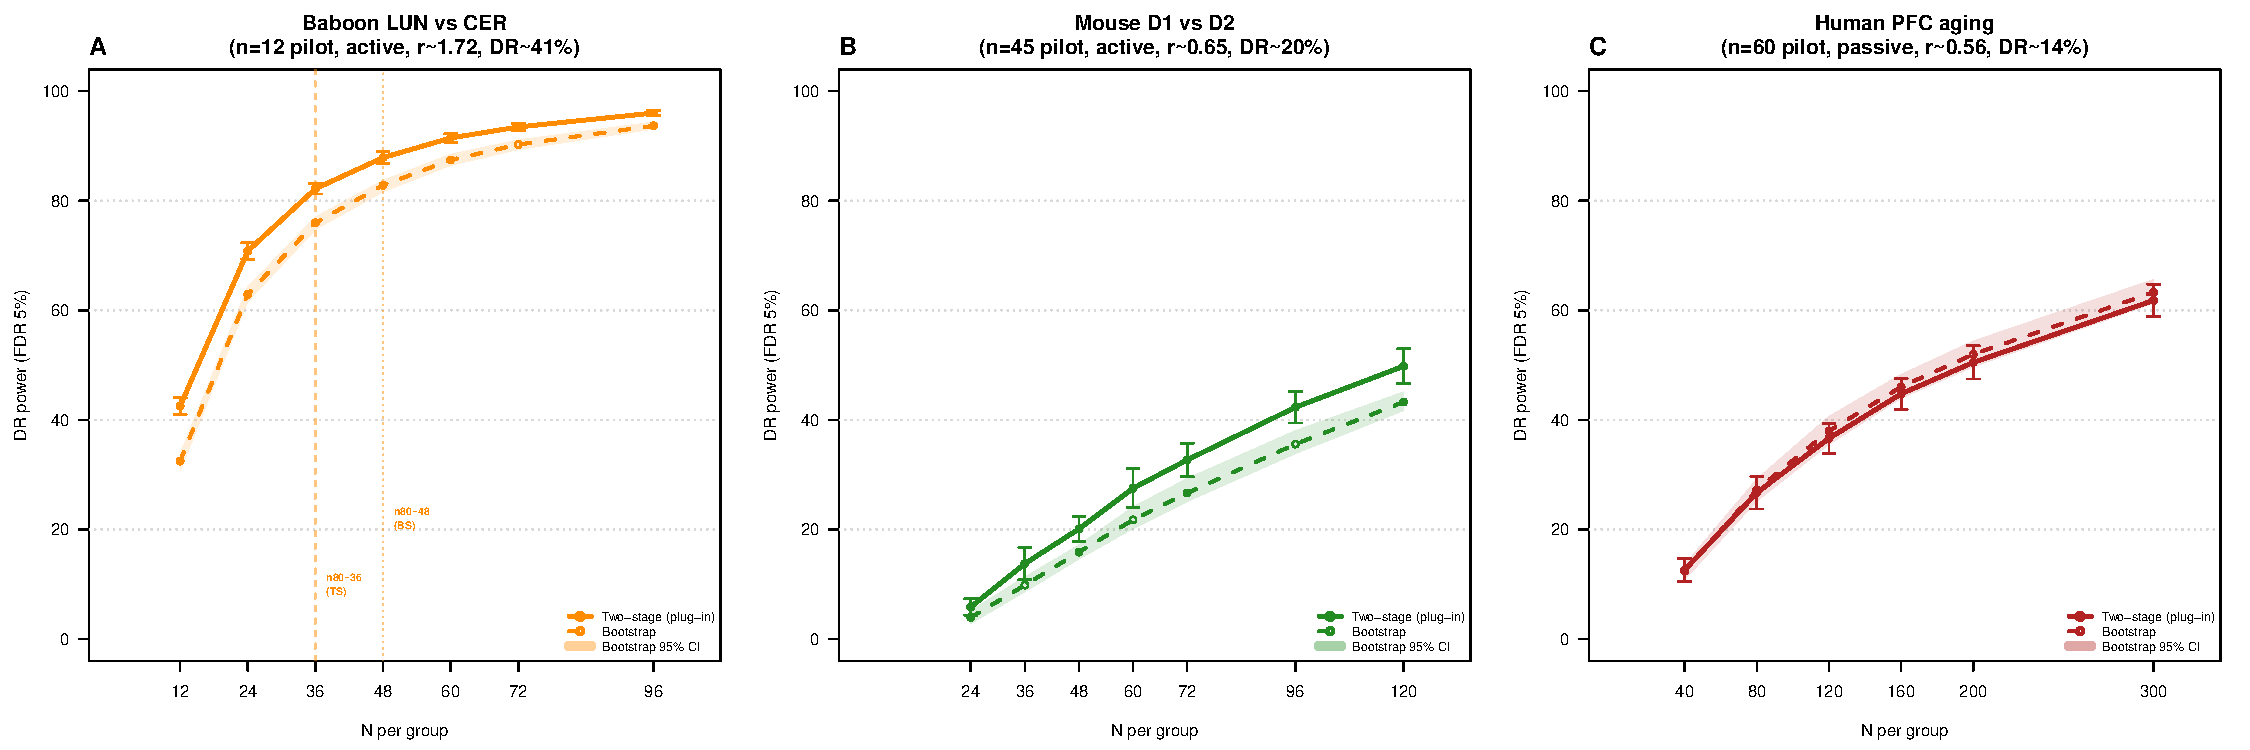
\includegraphics[width=\textwidth]{figures/bootstrap_summary.pdf}
\caption{Bootstrap vs.\ two-stage projected DR power across three pilot datasets.
Left: Baboon LUN vs.\ CER ($n=12$, active $B=12$, $m=1$).
Centre: Mouse D1 vs.\ D2 ($n=45$, active $B=6$).
Right: Seney MDD vs.\ Control ACC ($n=60$, passive).
Solid lines: two-stage plug-in power. Dashed lines: bootstrap mean power.
Shaded bands: 95\% bootstrap CI (pointwise). For Baboon, the plug-in
overestimates power by 5--7\,pp. CI width reflects pilot informativeness:
the active Baboon design ($B=12$, full 24\,h coverage) yields tighter
intervals than the passive Seney design despite a smaller pilot sample.}
\label{fig:bootstrap_baboon}
\end{figure}

\subsection{Active Design: Multi-Dataset Power and Effect-Size Scaling}

To evaluate \software{DiffCircaPower} across a wider range of study designs and effect sizes, we analyzed three additional pilot datasets spanning a 5-fold range in effect size. The mouse LIV vs.\ CER comparison (GSE54651; $n_{\text{pilot}} = 8$, $B = 8$, $m = 1$; Zhang et al.\ \cite{zhang2014comprehensive}) has median signal-to-noise ratio $\tilde{r} = 2.88$ and $\hat\pi_{\text{DR}} = 29.6\%$, representing the highest-signal scenario. The baboon LUN vs.\ CER comparison ($n_{\text{pilot}} = 12$, $B = 12$, $m = 1$) has $\tilde{r} = 1.72$ and $\hat\pi_{\text{DR}} = 40.7\%$. The mouse D1 vs.\ D2 striatal neuron comparison ($n_{\text{pilot}} = 45$, $B = 6$, $m \approx 7.5$) has $\tilde{r} = 0.65$ and $\hat\pi_{\text{DR}} = 19.9\%$ (Table~\ref{tab:signal_summary}).

\begin{table}[H]
\centering
\small
\begin{tabular}{lll|rrr}
\toprule
Dataset & Design & Tissue & $\tilde{r}$ & $\hat\pi_{\text{DR}}$ & $n_{\text{pilot}}$ \\
\midrule
Mouse LIV vs.\ CER \cite{zhang2014comprehensive} & Active, $B=8$, $m=1$ & Liver & 2.88 & 30\% & 8 \\
Baboon LUN vs.\ CER & Active, $B=12$, $m=1$ & Lung & 1.72 & 41\% & 12 \\
Mouse D1 vs.\ D2 & Active, $B=6$, $m\approx 8$ & Striatum & 0.65 & 20\% & 45 \\
Human PFC aging \cite{chen2016aging} & Passive & PFC & 0.56 & 14\% & 62 \\
\bottomrule
\end{tabular}
\caption{Pilot dataset characteristics ordered by effect size. $\tilde{r}$ = median signal-to-noise ratio across rhythmic genes; $\hat\pi_{\text{DR}}$ = estimated proportion of differentially rhythmic genes; $n_{\text{pilot}}$ = pilot sample size per group.}
\label{tab:signal_summary}
\end{table}

Effect size ($\tilde{r}$) is the primary determinant of required sample size (Figure~\ref{fig:multi_dr_power}). For mouse LIV vs.\ CER ($\tilde{r} = 2.88$), DR power reaches 80\% at $N \approx 24$--$28$ per group, confirming that strong liver rhythms require very modest sample sizes even with $m = 1$. For baboon ($\tilde{r} = 1.72$, $\hat\pi_{\text{DR}} = 41\%$), 80\% power is achieved at $N \approx 34$--$36$. For mouse D1D2 ($\tilde{r} = 0.65$, $\hat\pi_{\text{DR}} = 20\%$), power is substantially lower: even at $N = 150$ per group, DR power reaches only ${\sim}43\%$. Together with the human PFC result ($\tilde{r} = 0.56$, $n_{80} > 100$), these four datasets span a 5-fold range in $\tilde{r}$ and a $>$3-fold range in $\hat\pi_{\text{DR}}$, yielding $n_{80}$ estimates that differ by more than an order of magnitude. This reinforces the need for effect-size-aware, dataset-specific simulation rather than a one-size-fits-all power calculation.

\begin{figure}[H]
\centering
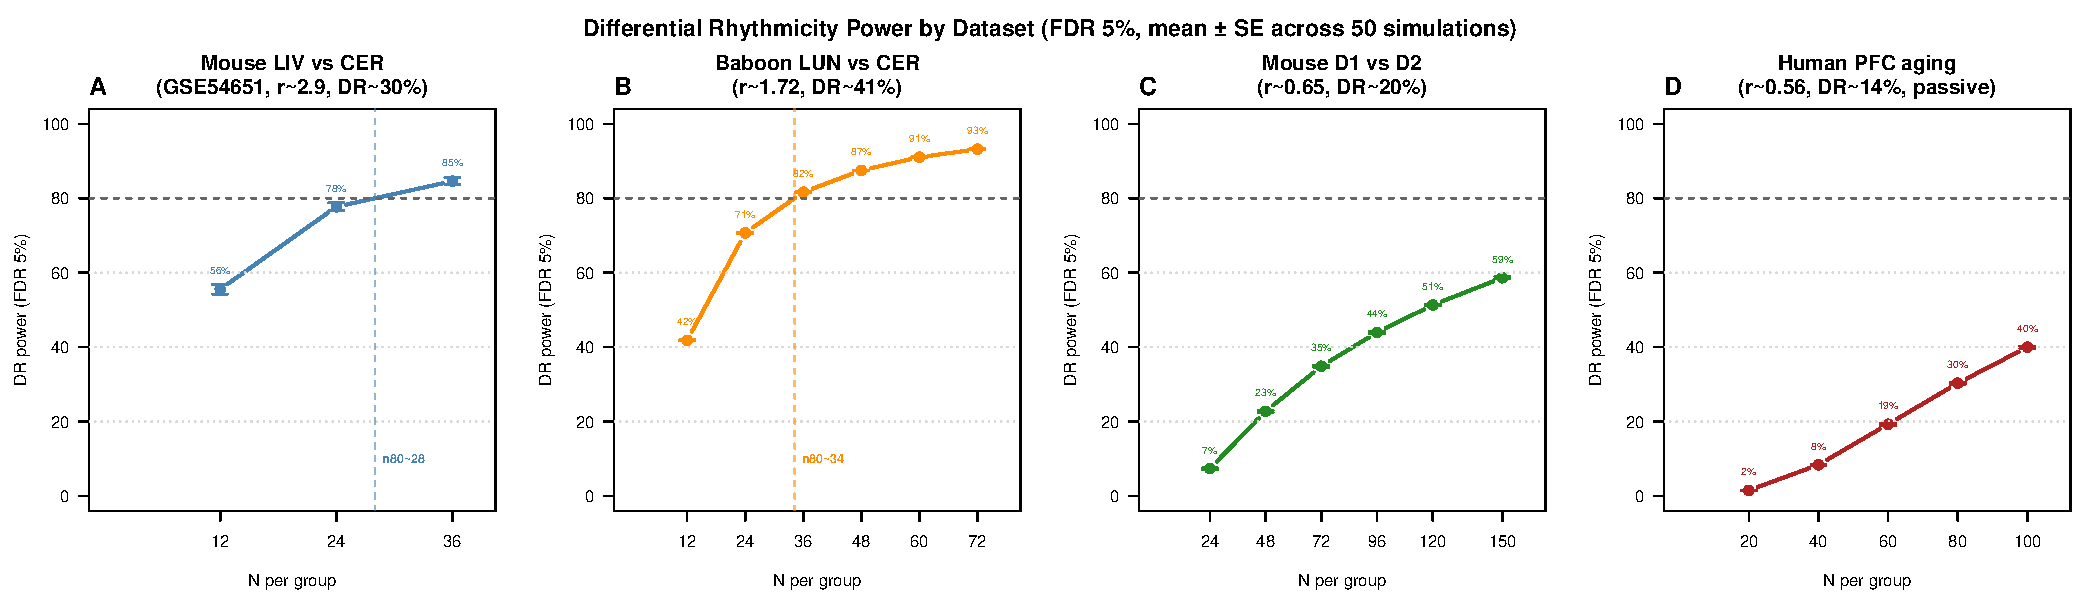
\includegraphics[width=\textwidth]{figures/multi_dataset_dr_power.pdf}
\caption{DR power vs.\ $N$ for four pilot datasets at FDR 5\% (mean $\pm$ SE across 50 simulations). Panels ordered by effect size (left to right: $\tilde{r} = 2.88$, $1.72$, $0.65$, $0.56$). Dashed line: 80\% power target. Vertical dashed line: interpolated $n_{80}$. The 5-fold range in $\tilde{r}$ translates to more than an order-of-magnitude difference in required sample size.}
\label{fig:multi_dr_power}
\end{figure}

\subsection{Maximizing Power: Time-Point Coverage vs.\ Replication}

For active designs, total sample size $N$ is allocated across $B$ distinct collection time points with $m = N/B$ replicates per time point. Here $B$ is the number of distinct time points and $m$ is the replication per time point. Proposition~1 (Section~\ref{sec:design_theory}) establishes that for a pure sinusoidal waveform, DR power depends only on $N$ (not on $B$), implying that B and m are interchangeable given fixed $N$. We evaluate this proposition empirically using bootstrap power grids over $(N, B)$ for the baboon and D1D2 datasets.

For the baboon dataset ($\tilde{r} = 1.72$), B-invariance holds approximately: DR power at $B = 6$ and $B = 12$ are within 1\,pp at all $N$ (e.g., $N = 60$: $B = 6$ gives 79.6\% [78.7\%, 80.3\%] vs.\ $B = 12$ gives 80.3\% [79.5\%, 80.9\%]). Both reach 80\% power at $N = 60$. Reducing to $B = 4$ incurs a 7--9\,pp penalty (73.6\% [72.8\%, 74.3\%] at $N = 60$), suggesting that $B = 4$ is insufficient to resolve the 24-h sinusoid precisely.

For the mouse D1D2 dataset ($\tilde{r} = 0.65$), the B effect is more pronounced: $B = 6$ gives more than twice the DR power of $B = 3$ at all tested $N$ (e.g., $N = 150$: $B = 6$ gives 42.8\% vs.\ $B = 3$ gives 18.3\%). This departure from B-invariance reflects the pilot data's real gene expression structure---including non-sinusoidal waveforms and temporal autocorrelation---which the pure-sinusoid simulation ($\alpha_2 = 0$) does not capture. In practice, denser temporal coverage ($B \geq 6$) improves cosinor model fit when $\tilde{r}$ is low and the sinusoidal assumption may not hold precisely.

To assess whether the cosinor model's sinusoidal assumption affects power projections, we simulated data with progressively non-sinusoidal waveforms by adding a second-harmonic component of strength $\alpha_2$ to the generating model (Supplementary Section~\ref{sec:fourier_robustness}; Figure~\ref{fig:fourier_robustness}). The results show that power projections are robust to moderate waveform distortion for $B \geq 4$: at $\alpha_2 = 0.5$ and $N \geq 48$, DR power loss is at most 2--9\,pp relative to the pure-sinusoid baseline. The cosinor assumption matters most when $m = 1$ (one sample per time point) and $N$ is small: without within-time-point replication, the model cannot separate waveform-induced residual variation from noise, and DR power collapses (e.g., from 58.6\% to 0.2\% at $N = 12$, $B = 12$ for Mouse LIV vs.\ CER). Together, these results support a practical design rule: use $B \geq 4$ evenly-spaced time points to protect against non-sinusoidal rhythms, and include at least $m = 2$ replicates per time point when $\tilde{r}$ is expected to be moderate or low or when $N$ is small.

\begin{figure}[H]
\centering

\includegraphics[width=\textwidth]{figures/bm_tradeoff.pdf}
\caption{B vs.\ m tradeoff across datasets (from left: Mouse LIV vs.\ CER, Baboon LUN vs.\ CER, Mouse D1 vs.\ D2). Each line is a $B$ value; shaded bands show 95\% bootstrap CIs. For the high-signal datasets (Mouse LIV, Baboon), $B$ and $m$ are approximately interchangeable for $B \geq 6$ (B-invariance holds). For the weak-signal D1D2 dataset, $B = 6$ substantially outperforms $B = 3$ at all $N$, demonstrating that denser temporal coverage is essential when $\tilde{r}$ is low.}
\label{fig:bm_tradeoff}
\end{figure}

\subsection{Differential Rhythmicity Power}

DR power was evaluated with 15\% of genes showing gain/loss of rhythm. Marginal per-gene power averages over all target genes and therefore reflects the full $r$ distribution. At FDR 5\%, marginal power ranges from 1.1\% ($n = 20$) to 30.5\% ($n = 100$), with empirical FDR well controlled (0.018--0.028; Table~\ref{tab:main_power}). The low marginal power reflects the predominance of low-$r$ genes in human brain tissue (Table~\ref{tab:effect_sizes}). Stratified analysis (Figure~\ref{fig:dr_power}) shows that genes with $r > 1.25$ achieve $\geq$83\% power at $n = 60$, while genes with $r < 0.5$ remain below 5\% power even at $n = 100$. Panel E shows that true discoveries are concentrated in higher-$r$ strata, and panel F shows the empirical distribution of DR targets across $r$ strata. Sensitivity to the nominal FDR threshold is shown in Figure~\ref{fig:dr_power}B,D.

\subsection{Differential Phase Power}

DP was evaluated with 15\% phase-shifted genes ($\pm$6\,h uniform). Marginal power averages over all target genes and thus reflects the full $r$ distribution. Marginal power reaches 68.7\% at $n = 100$ (Table~\ref{tab:main_power}), substantially higher than DR because phase-shifted genes retain rhythmicity in both groups. In the extended analysis (Figure~\ref{fig:dp_power}, panel C), marginal DP power exceeds 80\% at $n = 160$, indicating that DP becomes well powered at modestly larger sample sizes. Genes with $r > 0.75$ achieve $\geq$92\% power at $n = 60$ (Figure~\ref{fig:dp_power}). Panel E shows that true discoveries concentrate in moderate-to-high $r$ bins, and panel F shows the empirical distribution of DP targets across $r$ strata. Sensitivity to the nominal FDR threshold is shown in Figure~\ref{fig:dp_power}B,D.

\begin{table}[H]
\centering
\small
\begin{tabular}{r|rr|rr|rr}
\toprule
& \multicolumn{2}{c|}{FDR 5\%} & \multicolumn{2}{c|}{Emp.\ FDR} & \multicolumn{2}{c}{Avg TD} \\
$n$ & DR & DP & DR & DP & DR & DP \\
\midrule
20  & 1.1\%  & 13.3\% & 0.028 & 0.063 & 8   & 99  \\
40  & 5.4\%  & 34.5\% & 0.018 & 0.031 & 40  & 259 \\
60  & 13.1\% & 50.1\% & 0.020 & 0.024 & 98  & 376 \\
80  & 22.4\% & 61.4\% & 0.025 & 0.020 & 168 & 460 \\
100 & 30.5\% & 68.7\% & 0.021 & 0.023 & 229 & 515 \\
\bottomrule
\end{tabular}
\caption{Marginal power, empirical FDR, and average true discoveries for DR and DP tests (5,000 genes, 50 simulations, DCP method). Detailed results with standard errors in Supplementary Section~S1.}
\label{tab:main_power}
\end{table}

\begin{figure}[H]
\centering
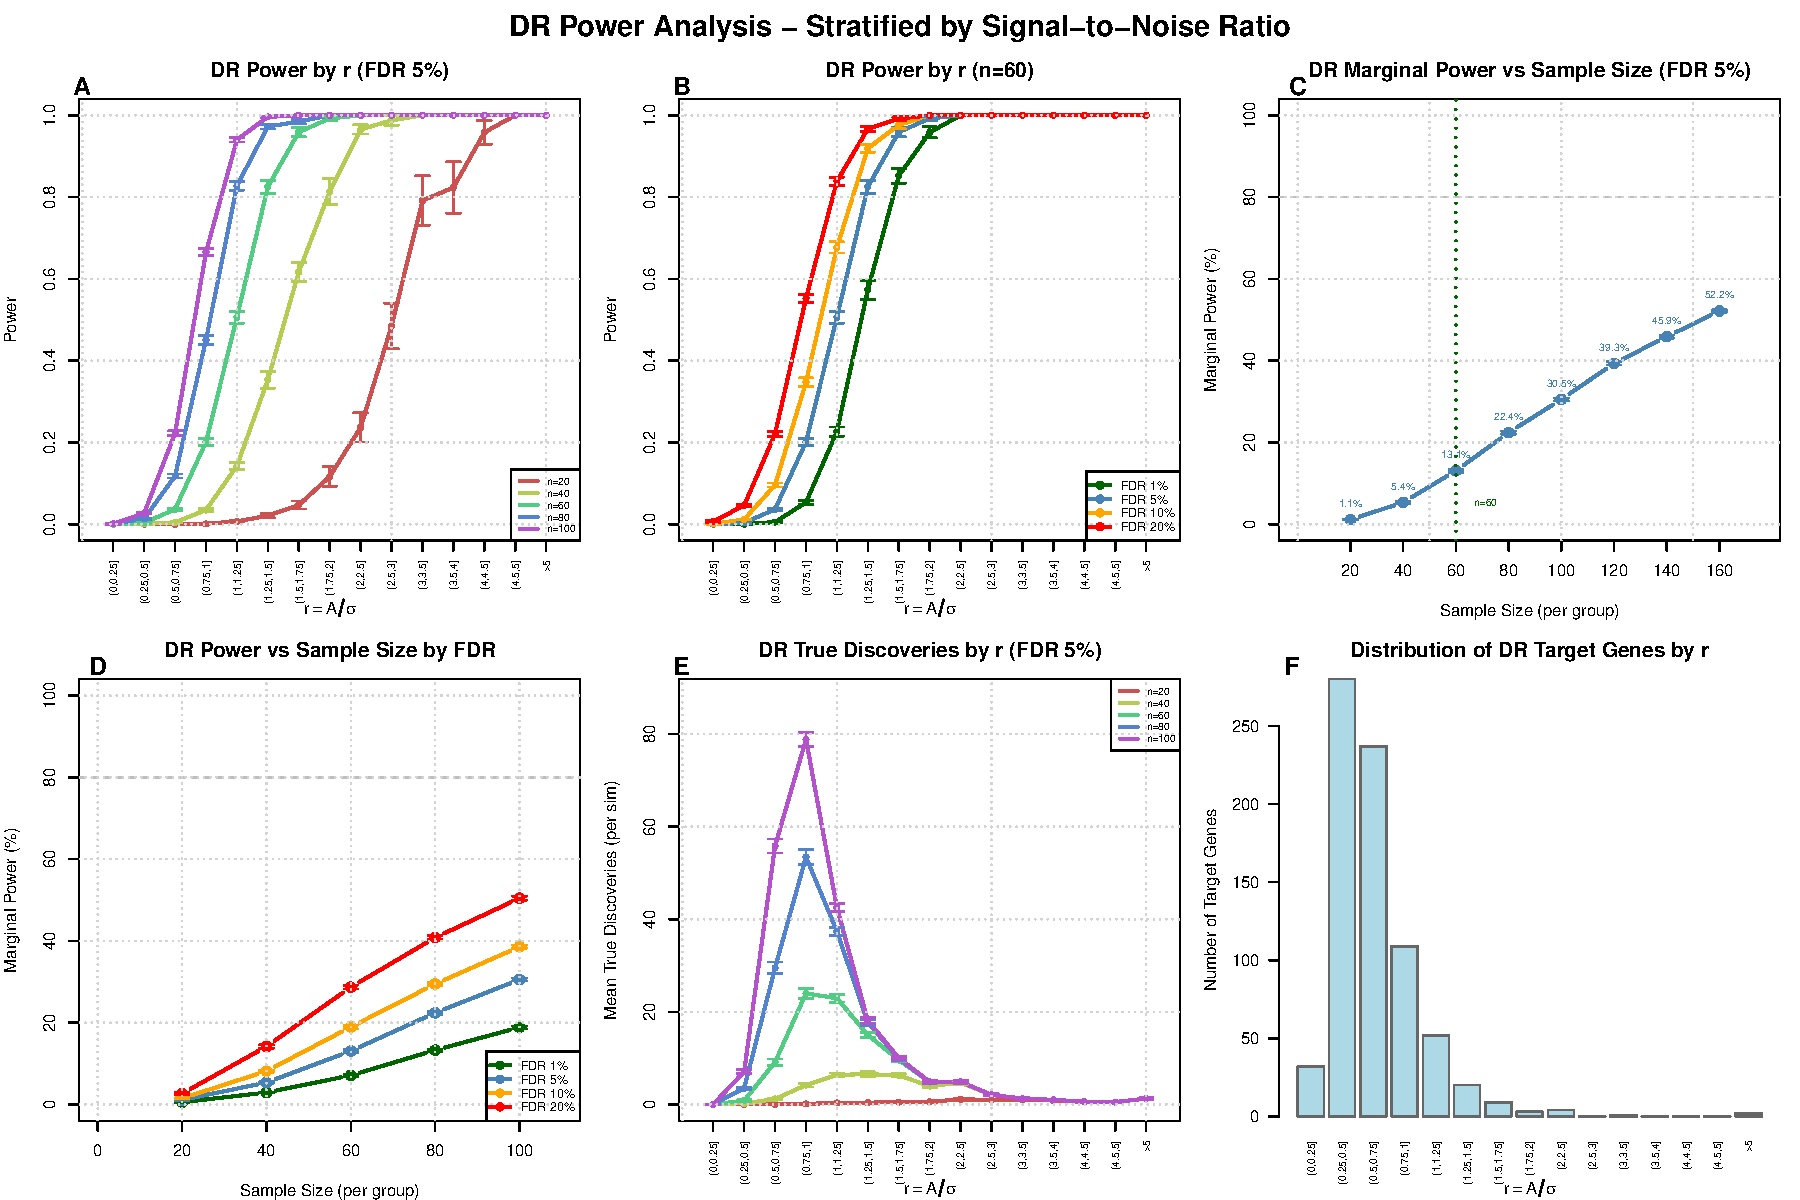
\includegraphics[width=\textwidth]{figures/dr_power.pdf}
\caption{DR power analysis. (A) Power by $r$ stratum at FDR 5\%. (B) Power by FDR threshold ($n=60$; sensitivity to nominal FDR). (C) Overall (marginal) per-gene power vs.\ sample size. (D) Overall (marginal) per-gene power by FDR threshold (sensitivity to nominal FDR). (E) True discoveries by $r$ stratum. (F) Empirical distribution of DR targets across $r$ strata.}
\label{fig:dr_power}
\end{figure}

\begin{figure}[H]
\centering
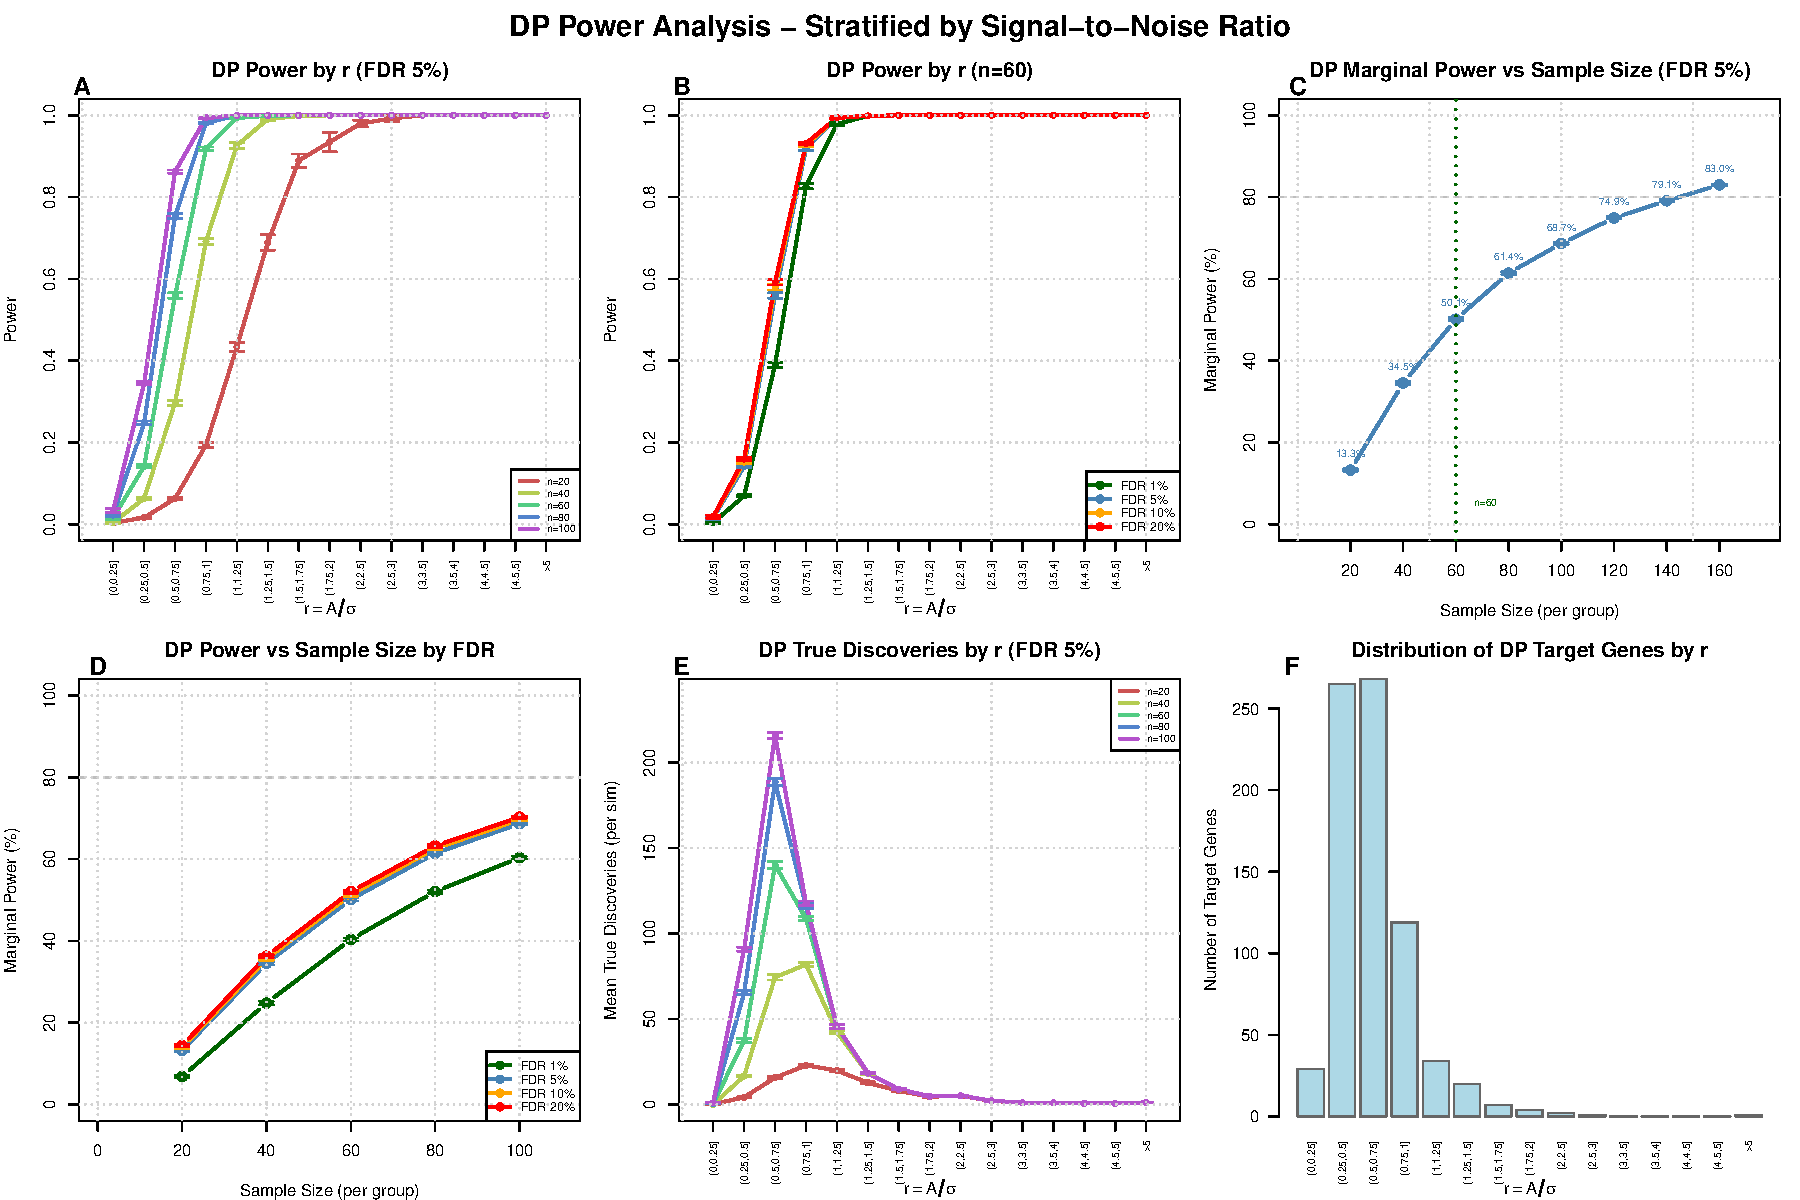
\includegraphics[width=\textwidth]{figures/dp_power.pdf}
\caption{DP power analysis ($\pm$6\,h phase shift). (B,D) show sensitivity to nominal FDR; (F) shows the empirical distribution of DP targets across $r$ strata. Panel layout otherwise matches Figure~\ref{fig:dr_power}.}
\label{fig:dp_power}
\end{figure}


\subsection{Phase Shift Sensitivity}

Power depends strongly on the magnitude of the phase difference (Figure~\ref{fig:phase_shift_abdf}), which motivates a sensitivity analysis based on the phase shift magnitude $\Delta\phi$ (hours). Because a 12\,h shift is anti-phase and maximal, $\Delta\phi$ is naturally bounded to $[0,12]$\,h. At $n = 60$, marginal power increases from 0.2\% (0.5\,h shift) to 39.0\% (4\,h) and 52.6\% (8\,h), then saturates beyond 8 hours (8\,h/12\,h power ratio $= 0.99$). Even at maximal (12\,h anti-phase) shifts, marginal power does not exceed 71.3\% ($n = 100$). Stratified analysis shows that genes with $r > 0.75$ achieve $\geq$80\% power for 4\,h shifts at $n = 60$ (Figure~\ref{fig:phase_shift_abdf}A). Full results are in Supplementary Section~S2.

\begin{figure}[H]
\centering
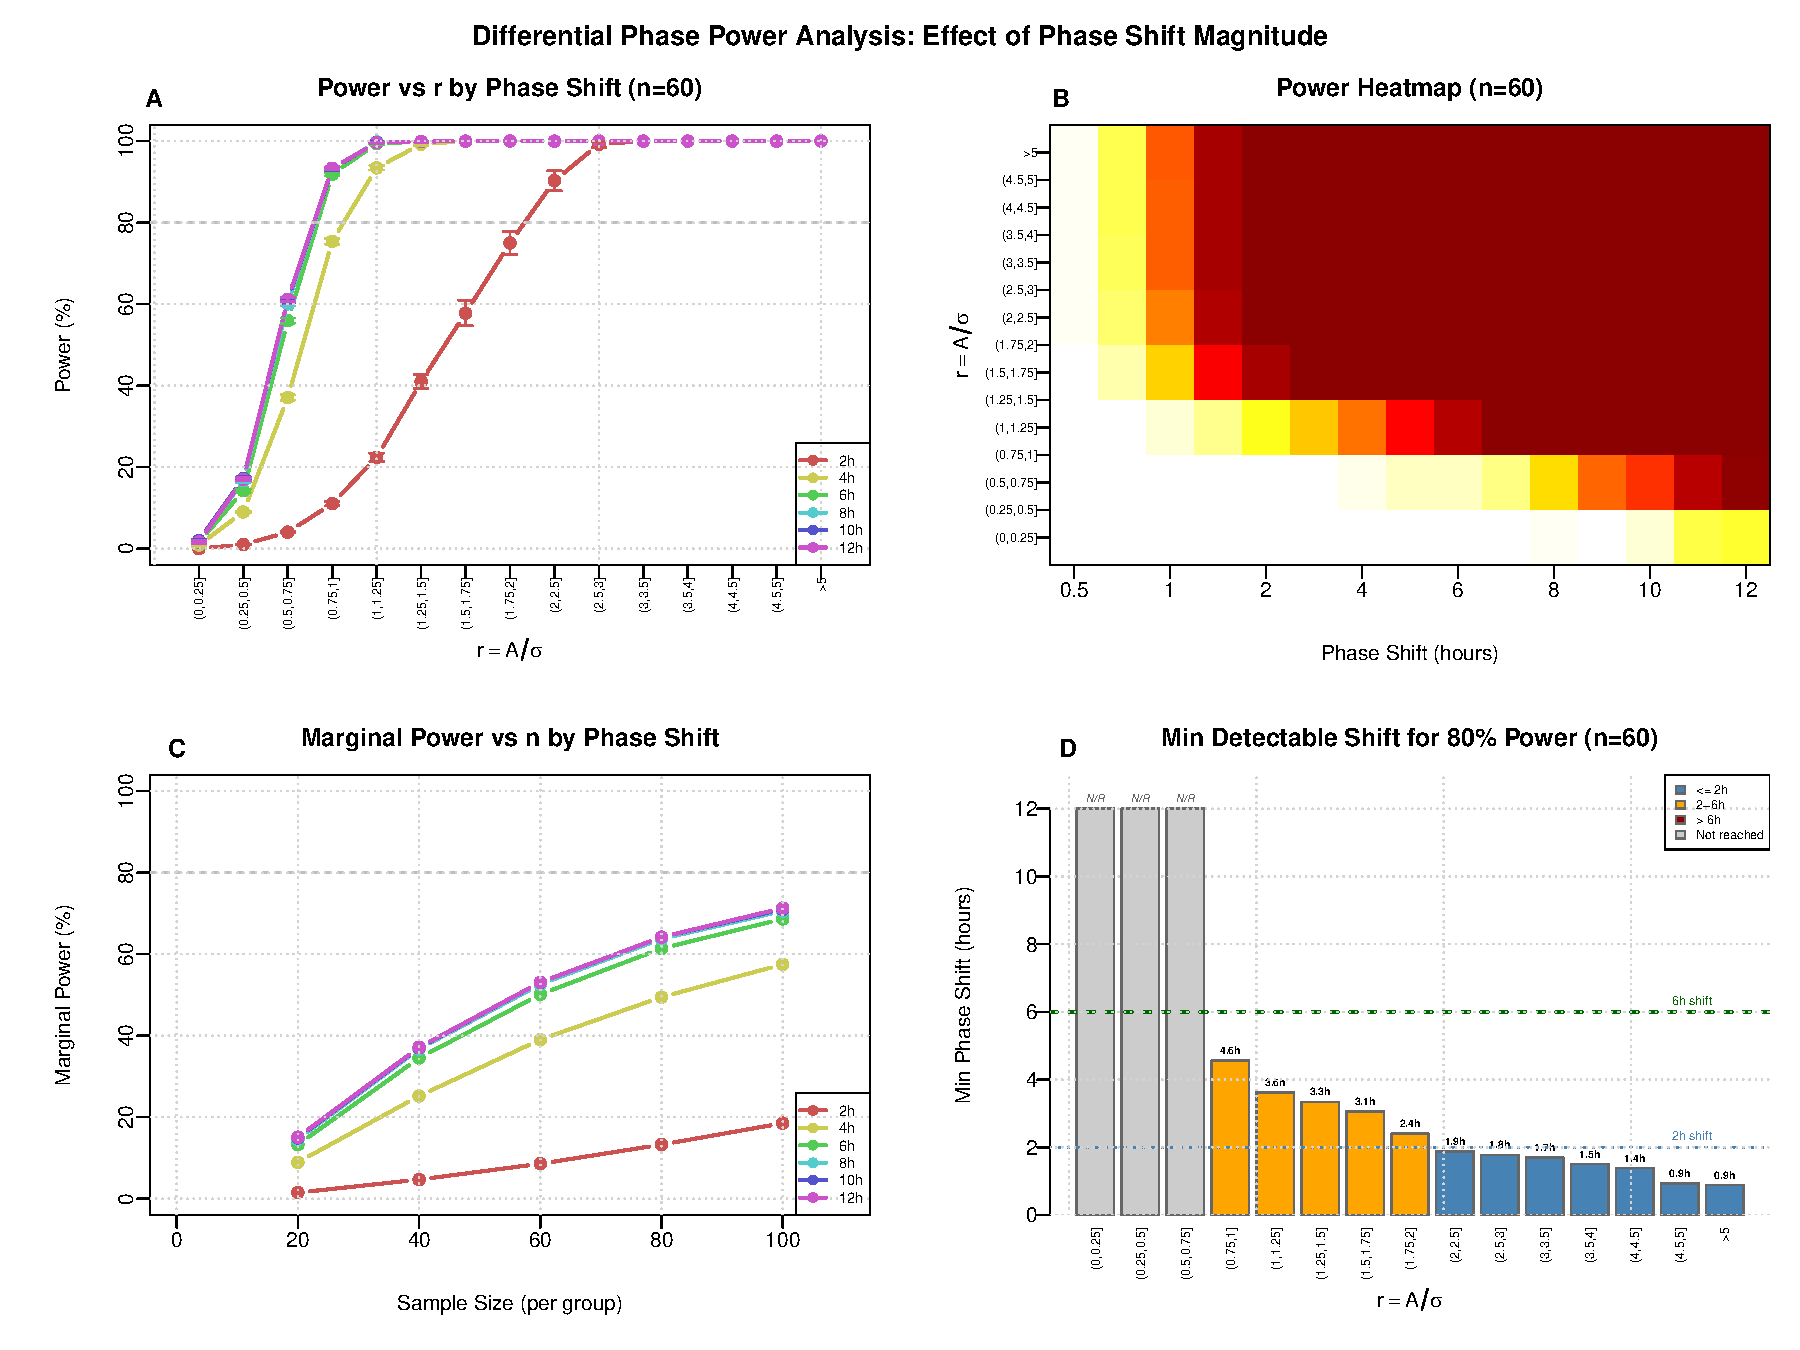
\includegraphics[width=\textwidth]{figures/phase_shift_abdf.pdf}
\caption{Phase shift sensitivity (5,000 genes, 50 simulations). (A) Power by $r$ stratum at $n=60$ across phase shifts. (B) Power heatmap ($r$ by phase shift). (C) Overall (marginal) per-gene power vs.\ sample size across phase shifts. (D) Minimum detectable phase shift by $r$ at $n=60$ (80\% power threshold).}
\label{fig:phase_shift_abdf}
\end{figure}

\subsection{Case Study: Comparing Detection Methods}

A key feature of \software{DiffCircaPower}'s modular architecture is its ability to evaluate competing detection methods on identical simulated data, enabling objective comparisons of power and false discovery rate (FDR). Methods such as \software{JTK\_CYCLE}, \software{RAIN}, and \software{MetaCycle} focus on rhythmicity detection and do not test individual circadian parameters. We therefore focus on \software{DiffCircaPipeline} (DCP) and \software{CircaCompare} (CC), which conduct gene-level inference on circadian parameters.

DCP and CircaCompare differ in both scope and statistical approach. DCP provides a complete differential analysis pipeline: it tests DR (gain/loss of rhythmicity) via a $\Delta R^2$ LRT, then tests DP among jointly rhythmic genes via constrained-MLE LRTs. CircaCompare tests per-parameter differences (DP and differential mesor) via Wald $t$-tests from per-gene NLS fits; it has no DR test equivalent because it lacks a $\Delta R^2$-type statistic for overall rhythm gain/loss. Thus, when DR is the primary question (e.g., identifying genes that lose rhythmicity in disease), DCP is the only available option.

For the shared test type (DP), we ran both methods on identical simulated datasets (Table~\ref{tab:method_comparison}; Figure~\ref{fig:method_comparison}). CircaCompare achieves 9--12 points higher DP power but at the cost of inflated FDR (8.7--19.6\% vs.\ nominal 5\%; Figure~\ref{fig:method_comparison}B), meaning a substantial fraction of apparent DP discoveries are false positives. DCP maintains proper FDR control across all sample sizes. For differential mesor (DM, no true effects), both methods control Type~I error ($<0.002$). Stratified comparison (Supplementary Section~S4) shows the power gap is concentrated in moderate-$r$ strata ($0.5 < r < 1.5$); at high $r$ both methods converge to near-perfect power.

The computational cost difference is also substantial: DCP processes $G = 5{,}000$ genes in ${\sim}2$\,s per simulation (vectorized via \texttt{limma}), while CircaCompare requires ${\sim}150$\,s (${\sim}0.03$\,s/gene $\times$ NLS). For a full power analysis with 50 simulations $\times$ 5 sample sizes, DCP completes in ${\sim}8$ minutes vs.\ ${\sim}10$ hours for CircaCompare.

\begin{table}[H]
\centering
\small
\begin{tabular}{r|cc|cc}
\toprule
& \multicolumn{2}{c|}{Power} & \multicolumn{2}{c}{FDR} \\
$n$ & DCP & CC & DCP & CC \\
\midrule
20  & 13.2 & 23.5 & .063 & .196 \\
40  & 34.5 & 46.8 & .031 & .127 \\
60  & 50.1 & 61.8 & .024 & .100 \\
80  & 61.4 & 71.3 & .020 & .090 \\
100 & 68.6 & 77.5 & .023 & .087 \\
\bottomrule
\end{tabular}
\caption{Method comparison (CC = CircaCompare) for DP. Power (\%, FDR 5\% threshold) and empirical FDR. CircaCompare achieves higher DP power but inflates DP FDR to 9--20\%.}
\label{tab:method_comparison}
\end{table}

\begin{figure}[H]
\centering
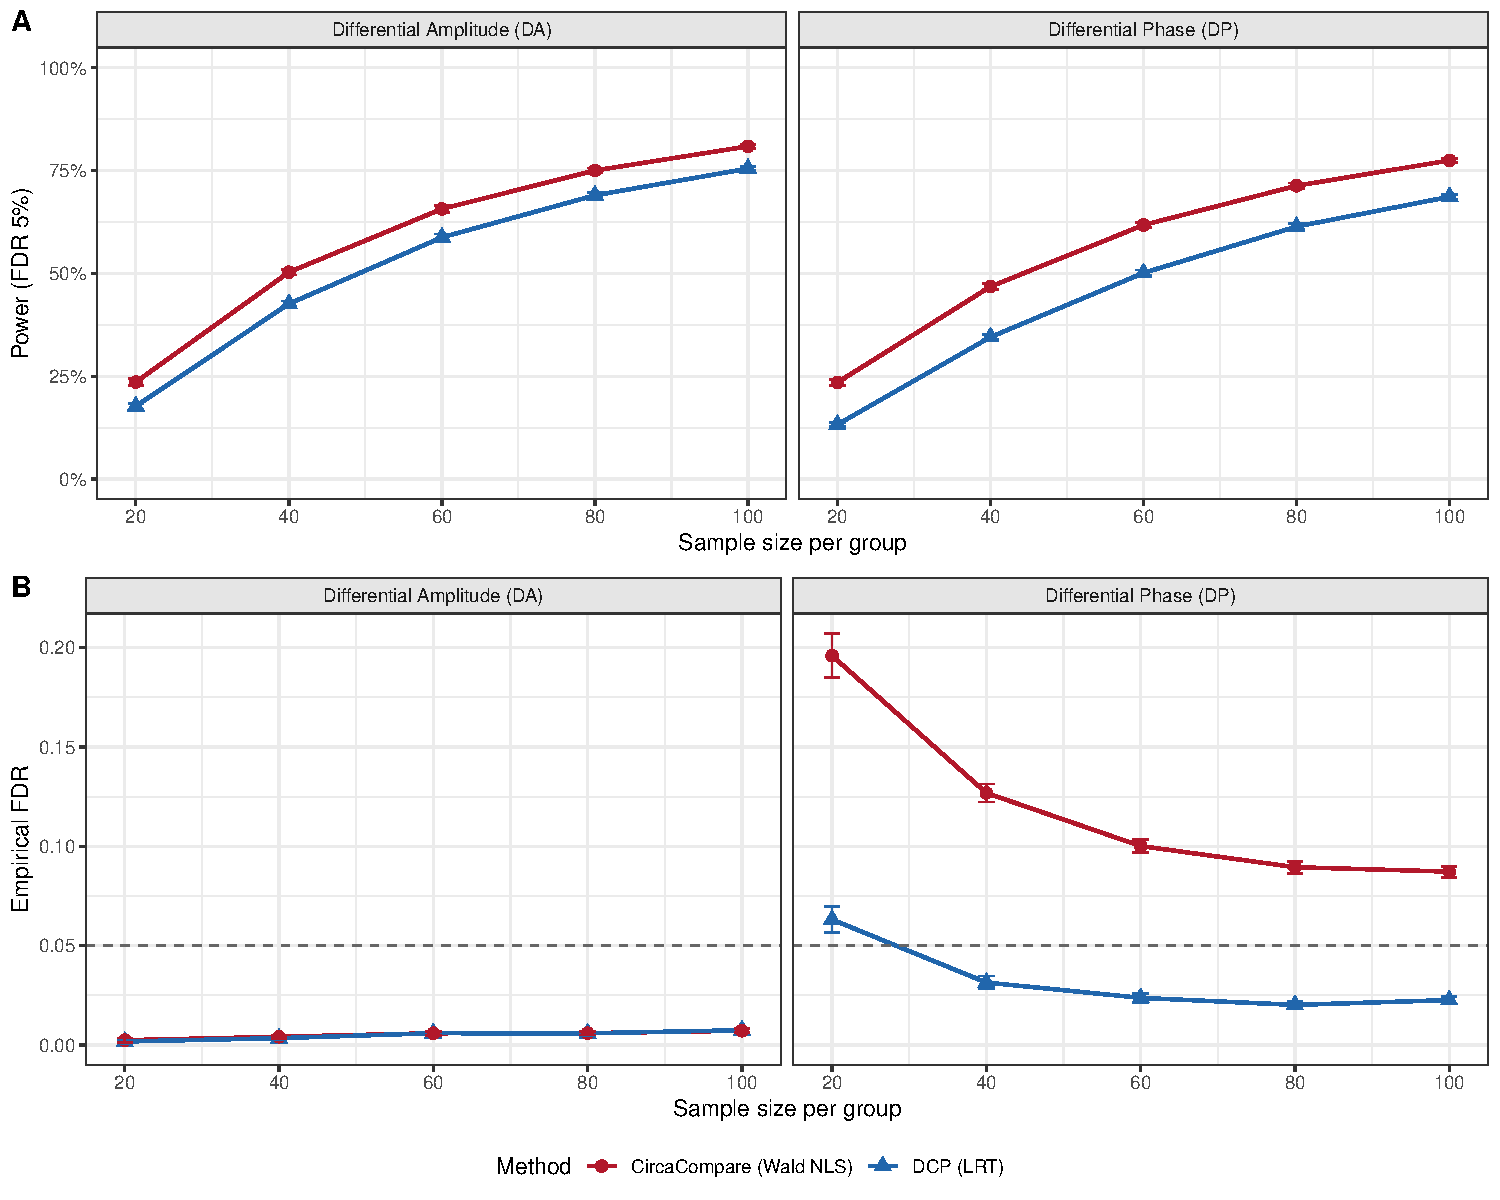
\includegraphics[width=\textwidth]{method_comparison/figures/method_comparison_combined.pdf}
\caption{Method comparison: DCP (LRT) vs.\ CircaCompare (Wald NLS) for DP. (A) Marginal power at FDR 5\%. CircaCompare achieves consistently higher power. (B) Empirical FDR. CircaCompare inflates FDR to 9--20\%, far above the nominal threshold (dashed line), while DCP maintains proper control. Error bars show $\pm$1.96 SE across 50 simulations.}
\label{fig:method_comparison}
\end{figure}

\subsection{Validation}

Framework validity was confirmed through four checks (details in Supplementary Section~S5). Under the complete null, raw $p$-value rejection rates are near nominal $\alpha = 0.05$ for DR (0.054--0.072) and DP (0.052--0.065); after BH correction the false positive rate is 0.000 for all tests, confirming multiple-testing control. Power increases monotonically with sample size for all tests and $r$-strata. Power also increases with phase shift magnitude and saturates near 8\,h. Empirical FDR is at or below nominal for DR (0.018--0.028) and DP (0.020--0.063), with slight inflation only at $n = 20$.

%% ====================================================================
\section{Discussion}
%% ====================================================================

Our simulation study yields five principal findings that are directly relevant to experimental design.

First, \textbf{DR detection is severely underpowered in human brain tissue}. Even at $n = 100$ per group, marginal DR power is only 30.5\%, driven by the low median effect size ($\tilde{r} = 0.556$) in post-mortem human brain. This is especially consequential for passive post-mortem studies, where samples are scarce, collection times are fixed, and design efficiency is reduced ($d \approx 0.24$ vs.\ $d = 0.5$ for active designs). Without simulation-based guidance, researchers risk committing years of tissue procurement to an underpowered study or missing the fact that targeted analysis of high-$r$ genes can yield reliable results with moderate sample sizes.

Second, \textbf{stratified power analysis is essential}. Marginal power averages across genes with heterogeneous effect sizes and masks dramatic variation: high-$r$ genes ($r > 1.25$) are reliably detected at $n = 60$ ($\geq$83\% DR power), while low-$r$ genes ($r < 0.5$) remain below 5\% power even at $n = 100$. This parallels PROPER's finding for RNA-seq \cite{wu2015proper}; in circadian data the disparity is especially large because the $r$ distribution spans a 50-fold range.

Third, \textbf{phase shift power saturates around 8 hours}. This reflects the geometric limit of cosine separation: for two cosines with identical $A$ and phase difference $\Delta\phi$, the squared amplitude of $y_1(t) - y_2(t)$ is proportional to $\sin^2(\pi\Delta\phi/\tau)$, which plateaus for $\Delta\phi > \tau/3 \approx 8$\,h.

Fourth, \textbf{the case study comparing DCP and CircaCompare illustrates how \software{DiffCircaPower} can guide method selection}. The two methods occupy complementary niches. DCP is the only tool providing a DR test for overall gain/loss of rhythmicity, making it indispensable when DR is the primary scientific question. For the shared test type (DP), CircaCompare offers 9--12 percentage points higher power but at the cost of inflated DP FDR (9--20\% vs.\ nominal 5\%) and ${\sim}75\times$ longer computation time. When the effective true discovery rate is adjusted for false positives, $\text{Power}_{\text{adj}} = \text{Power} \times (1 - \widehat{\text{FDR}})$, the DP gap narrows substantially (e.g., at $n = 60$: DCP $50.1\% \times 0.976 = 48.9\%$ vs.\ CC $61.8\% \times 0.900 = 55.6\%$). For DP, DCP is preferred in discovery studies where FDR control is critical, while CircaCompare may be considered when the power gain outweighs the inflation risk and findings will be independently validated. The computational difference is also practically relevant: a full power analysis across 50 simulations and 5 sample sizes completes in ${\sim}8$ minutes with DCP versus ${\sim}10$ hours with CircaCompare, making DCP far more suitable for exploratory analyses involving many scenarios. More broadly, this case study demonstrates how \software{DiffCircaPower}'s pluggable architecture enables evidence-based method choices by running competing methods on identical simulated data.

Fifth, \textbf{the two-stage plug-in method systematically overestimates projected power, and bootstrap resampling corrects this bias while quantifying pilot uncertainty}. By treating pilot parameter estimates as exact, the plug-in approach ignores the variability that would result from re-running the pilot study. On the baboon LUN pilot ($n = 12$ active samples), the plug-in recommendation was $\hat{n}_{80} = 36$, but at that sample size the bootstrap analysis shows projected power is only 76\% [74.8\%, 77.0\%]---a gap of 6\,pp that would result in an underpowered study. The bootstrap recommendation of $N = 48$ correctly accounts for this uncertainty. Crucially, tight bootstrap confidence intervals do not require a large pilot: the baboon design uses only 12 animals with $m = 1$ replicate per time point, yet CIs are $\leq 3$\,pp wide because 12 equally-spaced time points fully constrain the cosinor parameters. The key is design informativeness---an active design with full 24-h coverage---rather than pilot size per se.

\paragraph{B vs.\ m allocation and temporal resolution.} Proposition~1 establishes that for a pure sinusoidal waveform, DR power depends only on total sample size $N$ and not on how $N$ is split between time points $B$ and replicates per time point $m$. Empirically, we confirm this B-invariance across all datasets tested ($B \in \{3, 4, 6, 12\}$, $N \in \{12, 24, 48, 72\}$): when data are generated from a pure sinusoid ($\alpha_2 = 0$), DR power differs by $\leq 1$\,pp across all $B$ values at each $N$.

When the cosinor assumption is violated---that is, when the true waveform departs from a pure sinusoid (simulated here by adding a second-harmonic component of strength $\alpha_2 = 0.5$)---the allocation choice begins to matter, particularly at small $N$. Because the cosinor model fits only the fundamental frequency, non-sinusoidal components contribute unexplained residual variance, reducing effective $R^2$ and consequently DR power. This effect is most severe when $m = N/B = 1$ (no replication within time points): in the mouse GSE54651 dataset ($r = 2.9$), DR power at $N = 12$ collapses from 58.6\% to near zero (0.2\%) as $\alpha_2$ increases to 0.5 at $B = 12$. With $m \geq 2$ the impact is attenuated, and at $N \geq 48$ the power penalty is small ($\leq 2$\,pp). The practical implication is that single-replicate designs ($m = 1$), such as single-animal-per-time point studies, are sensitive to violations of the sinusoidal assumption at small total sample sizes. Adding even one replicate per time point ($m = 2$) substantially mitigates this vulnerability.

\paragraph{Practical recommendations.} For DR in human brain tissue: $n \geq 80$ for modest marginal per-gene power; targeted analyses of high-$r$ genes can succeed with $n = 40$--60. For DP ($\pm$6\,h shifts): $n = 60$ achieves 50\% marginal per-gene power. These recommendations are specific to human post-mortem brain, which has among the lowest circadian effect sizes of any tissue \cite{zong2023circapower} and therefore represents a conservative design baseline. For actively-designed mouse studies, where core-gene $r$ values are typically 3--10$\times$ higher ($r \approx 2$--$6$; CircaPower Table~1), substantially smaller sample sizes would suffice. Active designs also benefit from a higher design factor ($d = 0.5$ vs.\ ${\sim}0.24$ for passive), further reducing sample requirements. In all cases, we recommend reporting stratified alongside marginal per-gene power, as the latter can be misleading when $r$ is heterogeneous and can obscure actionable design guidance.

\paragraph{Why stratified power matters.} Marginal power averages over the full distribution of $r$ and is dominated by the large mass of low-$r$ genes in human brain, leading to uniformly low averages even when a subset of strong rhythms is well powered. Stratified power makes this heterogeneity explicit by reporting power within $r$-bins, showing which effect sizes are detectable at feasible $n$. This framing supports targeted study design: investigators can choose sample sizes based on the effect-size range that is biologically meaningful rather than a single marginal average.

\paragraph{Limitations.} Current limitations include: (i) independent marginal resampling of $\mu_g$, $\sigma_g$, and $A_g$ (ignoring potential correlations across genes; joint resampling of per-gene parameter tuples would preserve the empirical correlation structure); (ii) passive design results are specific to the pilot data's time-of-day distribution (different tissues or cohorts may have different $F_{\text{TOD}}$ and hence different $d$); (iii) computational cost of CircaCompare (${\sim}150$\,s per simulation vs.\ ${\sim}2$\,s for DCP) limits feasible $N_{\text{sim}}$; (iv) the cosinor model assumes sinusoidal waveforms; however, we evaluated this assumption by simulating data with increasing non-sinusoidal distortion (second-harmonic strength $\alpha_2 \leq 0.5$, which covers realistic bulk RNA-seq waveforms \cite{hughes2009harmonics}), and found power loss of at most 2--9 percentage points for $B \geq 4$ at $N \geq 48$, so this assumption is not consequential in practice for the study designs considered; and (v) BH control assumes independence or PRDS across genes, whereas gene--gene correlations may affect calibration in practice.

A further limitation is that differential gene types are modeled as mutually exclusive: each gene is assigned to exactly one of DR or DP, and compound changes (e.g., a gene that simultaneously shifts phase and loses rhythmicity, as commonly observed in aging or neuropsychiatric disease) are not simulated. In real transcriptomes, circadian disruption often manifests as correlated multi-parameter changes rather than isolated single-parameter shifts. However, simulating each differential type in isolation is the standard approach in power analysis for multi-parameter tests, for the same reason that DE power analysis evaluates fold-changes in isolation: it allows clean, interpretable power curves for each test type and avoids confounding from compound effects that would make it impossible to attribute detection to a specific test. The one-at-a-time design is therefore appropriate for the primary goal of guiding study design, where investigators typically need to know the power for a specific hypothesis (e.g., ``how many subjects to detect phase-shifted genes?'') rather than the power under a complex joint model. Future work could extend the framework to compound-type genes to evaluate robustness of test specificity under realistic multi-parameter disruption.

\paragraph{Software availability.} \software{DiffCircaPower} is available as an open-source R framework with a PROPER-style configuration system. An end-to-end pipeline (\texttt{examples/run\_pipeline.R}) reproduces all results in this paper, and a validation suite (\texttt{examples/run\_validation.R}) implements the checks described in Section~3.6.

\section*{Acknowledgments}

This work builds on \software{CircaPower} \cite{zong2023circapower}, \software{PROPER} \cite{wu2015proper}, \software{DiffCircaPipeline} \cite{xue2023diffcircapipeline}, and \software{CircaCompare} \cite{parsons2020circacompare}.

\bibliographystyle{plain}
\bibliography{references}

\end{document}
